\documentclass[a4paper,12pt,twoside]{scrreprt}
% Autor der Vorlage: Klaus Rheinberger, FH Vorarlberg
% 2017-02-20

%% Hilfe: z.B.
% empfohlener Einstieg: http://latex.tugraz.at/  
% https://de.wikibooks.org/wiki/LaTeX-Kompendium:_Schnellkurs:_Erste_Schritte
% https://de.wikibooks.org/wiki/LaTeX-Kompendium:_Schnellkurs
% https://de.wikibooks.org/wiki/LaTeX-Kompendium

%% Pakete:
% Der Befehl \usepackage[latin9]{inputenc} ermöglicht die direkte Angabe von Umlauten. Übrigens lässt sich so auch das Euro-Zeichen direkt eingeben. Auf Betriebssystemen, wie zum Beispiel allen neueren Linux-Distributionen, verwendet man statt \usepackage[latin9]{inputenc} besser \usepackage[utf8]{inputenc}, auf Applesystemen verwendet man \usepackage[macce]{inputenc} (oder das für ältere Modelle gültige \usepackage[applemac]{inputenc}).
\usepackage[utf8]{inputenc}
\usepackage[T1]{fontenc}    % Silbentrennung bei Sonderzeichen
\usepackage{graphicx}       % Bilder einbinden
\usepackage{lscape}         % Querformat
\usepackage{pdfpages}
\usepackage[ngerman]{babel} % Deutsche Sprachanpassungen
\usepackage{footnote}       % footer citations
\usepackage{csquotes}       % When using babel or polyglossia with biblatex, loading csquotes is recommended to ensure that quoted texts are typeset according to the rules of your main language.
\usepackage{acronym}  % für optionales Abkürzungsverzeichnis
\usepackage[linktocpage=true]{hyperref} % Links z. B. \href{https://www.wikibooks.org}{Wikibooks home}
\usepackage{caption} % Abbildungslegenden
\usepackage{booktabs} % schönere horizontale Trennlinien für Tabellen 
\captionsetup{format=hang, justification=raggedright}
\usepackage[style=verbose,backend=bibtex]{biblatex}   % Literaturverweise
% biblatex comes with a variety of built-in bibliography/citation style families (numeric, alphabetic, authoryear, authortitle, verbose), and there's a growing number of custom styles:
% https://de.sharelatex.com/learn/Biblatex_citation_styles
% https://de.sharelatex.com/learn/Biblatex_bibliography_styles
\addbibresource{bibliography.bib}    % Zotero-Beispiele.bib ist die verwendete Bibtex-Datei 
% Anstatt die Bibtex-Datei selber zu erstellen, kann sie z. B. aus einer Zotero-Sammlung zu BibTeX exportiert werden.

% float package
\usepackage{float}

% fußnotennummerierung nicht neu beginnen in jedem kapitel
\usepackage{chngcntr}
\counterwithout*{footnote}{chapter}

% enumitem for enumarations
\usepackage{enumitem}
\setlist[1]{itemsep=0pt,parsep=0px}

% use for side-by-side figures
\usepackage{subfigure}

%% Einstellungen:
\setcounter{secnumdepth}{4}
\setcounter{tocdepth}{4}   % Tiefe der Gliederung im In haltsverzeichnis


%% ERSETZEN VON ECKIGEN KLAMMERN:
% Ersetzen Sie den Text in den eckigen Klammern!

\begin{document}

% Titelblatt:
% \newpage\mbox{}\newpage

% force output to a right page
\cleardoublepage{}
\thispagestyle{empty}
\begin{titlepage}
  \begin{flushright}
  
\includegraphics[width=0.4\linewidth]{Logo-A3}
  \end{flushright}
  \begin{flushleft}
  \section*{Agile Metriken}
  \subsection*{Qualitätssicherung in agilen Teams}
  \vspace{1.5cm}
  
  Masterarbeit\\
  zur Erlangung des akademischen Grades
  \vspace{0.5cm}
  
  \textbf{Master of Science (MSc)}

  \vspace{2cm}
  Fachhochschule Vorarlberg\newline
  Informatik

  \vspace{1cm}
  
  Betreut von\newline
  Prof.\ Dr.\ Michael Felderer
  
  \vspace{2cm}
  
  Vorgelegt von\newline
  Daniel Grießer\newline
  Dornbirn, Juli 2018
  \end{flushleft}
\end{titlepage}

% Kurzreferat:
\newpage
\section*{Kurzreferat}

\subsection*{[Deutscher Titel Ihrer Arbeit]}

[Text des Kurzreferats]


% Abstract:
\newpage
\section*{Abstract}
\subsection*{[English Title of your thesis]}

[text of the abstract]


% Inhaltsverzeichnis:
\cleardoublepage\tableofcontents

\clearpage
\phantomsection\addcontentsline{toc}{chapter}{Abbildungsverzeichnis}
\listoffigures

\clearpage
\phantomsection\addcontentsline{toc}{chapter}{Tabellenverzeichnis}
\listoftables

% Abkürzungsverzeichnis:
\clearpage
\phantomsection\addcontentsline{toc}{chapter}{Abkürzungsverzeichnis}
\chapter*{Abkürzungsverzeichnis}
\begin{acronym}
    \acro{APM}{Application-Performance-Monitoring}
    \acro{BI}{Business-Intelligence}
    \acro{CD}{Continuous Delivery}
    \acro{CI}{Continuous Integration}
    \acro{CLOC}{Changed Lines of Code}
    \acro{DoD}{Definition of Done}
    \acro{EAT}{Executive Action Team}
    \acro{EMS}{Executive Meta Scrum}
    \acro{FCM}{Factor Criteria Metrics}
    \acro{GQM}{Goal Question Metric}
    \acro{IEEE}{Institute of Electrical and Electronics Engineers}
    \acro{LeSS}{Large Scale Scrum}
    \acro{LOC}{Lines of Code}
    \acro{MTTF}{Mean Time to Failure}
    \acro{MTTR}{Mean Time to Release}
    \acro{NASA}{National Aeronautics and Space Administration}
    \acro{NoSQL}{Not-only-SQL}
    \acro{PBR}{Product Backlog Refinement}
    \acro{PTS}{Project Tracking System}
    \acroplural{PTS}[PTS]{Project Tracking Systems}
    \acro{QS}{Qualitätssicherung}
    \acro{SoS}{Scrum of Scrums}
    \acro{VCS}{Version Control System}
    \acroplural{VCS}[VCS]{Version Control Systems}
\end{acronym}


%% Die Kapitelstruktur ist mit der Betreuungsperson abzustimmen!
\chapter{Einleitung}

Dieses Kapitel gibt eine kurze Übersicht über den Aufbau und die Motivation hinter dieser Arbeit.

\section{Zielsetzung}

Agile Prozesse, insbesondere Scrum, basieren auf empirischen, also durch fortlaufende Beobachtung erhobenen und auswertenden, Daten (siehe Abschnitt~\ref{section:scrum}).
Das bedeutet, dass sich der Prozess durch Reflexion verbessert und auch Veränderung zulässt.
Um diese Reflexion zu vereinfachen, ist es hilfreich, gewisse Kennzahlen des Prozesses und des Produktes grafisch darzustellen.
Im Speziellen Metriken können eine gute qualitative Auskunft über den aktuellen Status geben.
Ziel dieser Arbeit soll es sein, Metriken zu ermitteln, die Qualitätsprobleme im Entwicklungsprozess oder im Softwareprodukt quantitativ abbilden können.
Weiters sollen diese Metriken gesammelt und grafisch dargestellt werden.
Sie können aus Daten generiert werden, die bei der tagtäglichen Arbeit in den jeweiligen Systemen erzeugt werden.
Solche Systeme reichen von \acfp{VCS}, über \acfp{PTS} und \acf{CI} / \acf{CD}, bis hin zu \acf{APM}.
Diese Daten können meist über Schnittstellen abgefragt und anschließend aggregiert abgelegt werden.
Umgesetzt wird das Ganze in einem relativ jungen, aber im Scrum Prozess bereits weit fortgeschrittenen Scrum-Team.

\clearpage
\section{Aufbau der Arbeit}

Nach der Einleitung gibt das Kapitel ``Stand der Technik'' einen Einblick in die unterschiedlichen Themen und die theoretischen Hintergründe dieser Arbeit.
Zuerst werden die Grundsäulen der agilen Softwareentwicklung, das agile Manifest und die agilen Prinzipien, genauer erklärt.
Darauf folgend wird auf Scrum eingegangen und zusätzlich Ansätze für Scrum in mehreren Teams erklärt.
Anschließend wird zu Qualität übergegangen, im Speziellen Software- und Prozessqualität.
Basierend auf den beiden vorherigen Themen, wird dann genauer auf Metriken eingegangen, was auch der Hauptteil dieses Kapitels darstellt.
Im ersten Teil werden Metriken aus den unterschiedlichsten Systemen vorgestellt und wie eigene Metriken erstellt werden können.
Danach folgen Hinweise zur Veröffentlichung von Metriken und der Messung von Agilen Prinzipien.
Am Schluss folgen noch ein Überblick über Qualitätsmodelle und das \ac{GQM}-Modell, sowie das \ac{FCM}-Modell im Detail.
\\
Im Kapitel ``Vorgehensweise'' wird beschrieben, wie bei der Bestimmung der relevanten Metriken für das Team, bei der Erstellung der Software und bei der Evaluierung der Ergebnisse vorgegangen wird.
\\
Das Kapitel ``Umsetzung'' zeigt dann, wie der Titel schon sagt, die Umsetzung der Lösung.
Anfangs werden die Gegebenheiten erläutert, in der die Lösung eingesetzt wird.
Dann wird mit der Identifizierung der Metriken gestartet und diese anschließend in der entwickelten Software gesammelt.
Zuletzt wird noch genauer auf die Darstellung eingegangen.
\\
Es folgt das Kapitel ``Evaluierung'', in dem die Ergebnisse qualitativ in Form von Interviews und quantitativ in Form der Metriken evaluiert werden.
In den Kapiteln ``Schlussfolgerungen'' und ``Zusammenfassung'' werden die Ergebnisse nochmal reflektiert, zusammengefasst und ein Ausblick für mögliche weitere Arbeiten gegeben.

\chapter{Stand der Technik}

Um eine Übersicht über die unterschiedlichen Themen zu bieten, werden im Folgenden die theoretischen Hintergründe dieser Arbeit näher erörtert.
Eine Übersicht am Anfang soll einen Einblick in die agile Softwareentwicklung gegeben.
Darauf folgend wird etwas genauer Scrum und die möglichen Varianten bei mehreren Teams erläutert.
Als Übergang dient eine kurze Aufarbeitung des Themas Software-Qualität, bevor die unterschiedliche Metriken im Detail erklärt werden.
Am Ende folgt noch eine Beschreibung von Qualitätsmodellen, im Speziellen das \ac{FCM}-Modell und zuletzt als Ergänzung noch die \ac{GQM}-Methodik.

\section{Agile Softwareentwicklung}

Diese Arbeit beschäftigt sich mit agilen Teams, deshalb ist es essentiell, zu verstehen, was der Gedanke hinter dem agilen Entwicklungsansatz ist.
Seinen Ursprung hat das Ganze im Jahr 2001, als sich ein paar schlaue Köpfe zusammengeschlossen haben und das sogenannte agile Manifest, sowie die agilen Prinzipien aufgestellt haben.
Ziel war es, eine Alternative zu den bisherigen, schwergewichtigen und von Dokumentation getriebenen Softwareentwicklungs-Methodologien zu finden.

\subsection{Agiles Manifest}

Das agile Manifest ist der Grundbaustein aller agilen Vorgehensmodelle:

\begin{quote}Wir erschließen bessere Wege, Software zu entwickeln,
indem wir es selbst tun und anderen dabei helfen.
Durch diese Tätigkeit haben wir diese Werte zu schätzen gelernt: \newline
\begin{center}
Individuen und Interaktionen mehr als Prozesse und Werkzeuge \newline
Funktionierende Software mehr als umfassende Dokumentation \newline
Zusammenarbeit mit dem Kunden mehr als Vertragsverhandlungen \newline
Reagieren auf Veränderung mehr als das Befolgen eines Plans \newline
\end{center}
Das heißt, obwohl wir die Werte auf der rechten Seite wichtig finden,
schätzen wir die Werte auf der linken Seite höher ein.\end{quote}\cite{agile_manifest}

\subsection{Agile Prinzipien}

Die agile Softwareentwicklung folgt diesen zwölf Prinzipien:

\begin{quote}Unsere höchste Priorität ist es, den Kunden durch frühe und kontinuierliche Auslieferung wertvoller Software zufrieden zu stellen.

Heisse Anforderungsänderungen selbst spät in der Entwicklung willkommen. Agile Prozesse nutzen Veränderungen zum Wettbewerbsvorteil des Kunden.

Liefere funktionierende Software regelmäßig innerhalb weniger Wochen oder Monate und bevorzuge dabei die kürzere Zeitspanne.

Fachexperten und Entwickler müssen während des Projektes täglich zusammenarbeiten.

Errichte Projekte rund um motivierte Individuen. Gib ihnen das Umfeld und die Unterstützung, die sie benötigen und vertraue darauf, dass sie die Aufgabe erledigen.

Die effizienteste und effektivste Methode, Informationen an und innerhalb eines Entwicklungsteams zu übermitteln, ist im Gespräch von Angesicht zu Angesicht.

Funktionierende Software ist das wichtigste Fortschrittsmaß.

Agile Prozesse fördern nachhaltige Entwicklung. Die Auftraggeber, Entwickler und Benutzer sollten ein gleichmäßiges Tempo auf unbegrenzte Zeit halten können.

Ständiges Augenmerk auf technische Exzellenz und gutes Design fördert Agilität.

Einfachheit -\phantom{}- die Kunst, die Menge nicht getaner Arbeit zu maximieren -\phantom{}- ist essenziell.

Die besten Architekturen, Anforderungen und Entwürfe entstehen durch selbstorganisierte Teams.

In regelmäßigen Abständen reflektiert das Team, wie es effektiver werden kann und passt sein Verhalten entsprechend an.\end{quote}\cite{agile_principles}

\clearpage
\section[Scrum]{Scrum~\footcite[vgl.][S.13ff]{scrum_kurz_gut_2013}}\label{section:scrum}

Das Scrum Framework ist eine solche agile Softwareentwicklungs-Methodologie. 
Scrum basiert auf Empirismus, also der Theorie, dass Wissen aus Erfahrung gewonnen wird und Entscheidungen auf Basis dieses Wissens getroffen werden. 
Die drei Grundsäulen einer solchen empirischen Prozesskontrolle sind:

\begin{description}
  \item[Transparenz] \hfill \\ Signifikante Aspekte des Prozesses müssen für alle sichtbar sein.
  \item[Inspektion] \hfill \\ Artefakte müssen regelmäßig inspiziert werden, aber dieser Vorgang darf der Arbeit selbst nicht im Weg stehen.
  \item[Adaption] \hfill \\ Weichen ein oder mehrere Aspekte eines Prozesses von seinen akzeptablen Limits ab, muss dieser so früh wie möglich angepasst werden.
\end{description}

\begin{savenotes}
  \begin{figure}[H] 
    \centering
    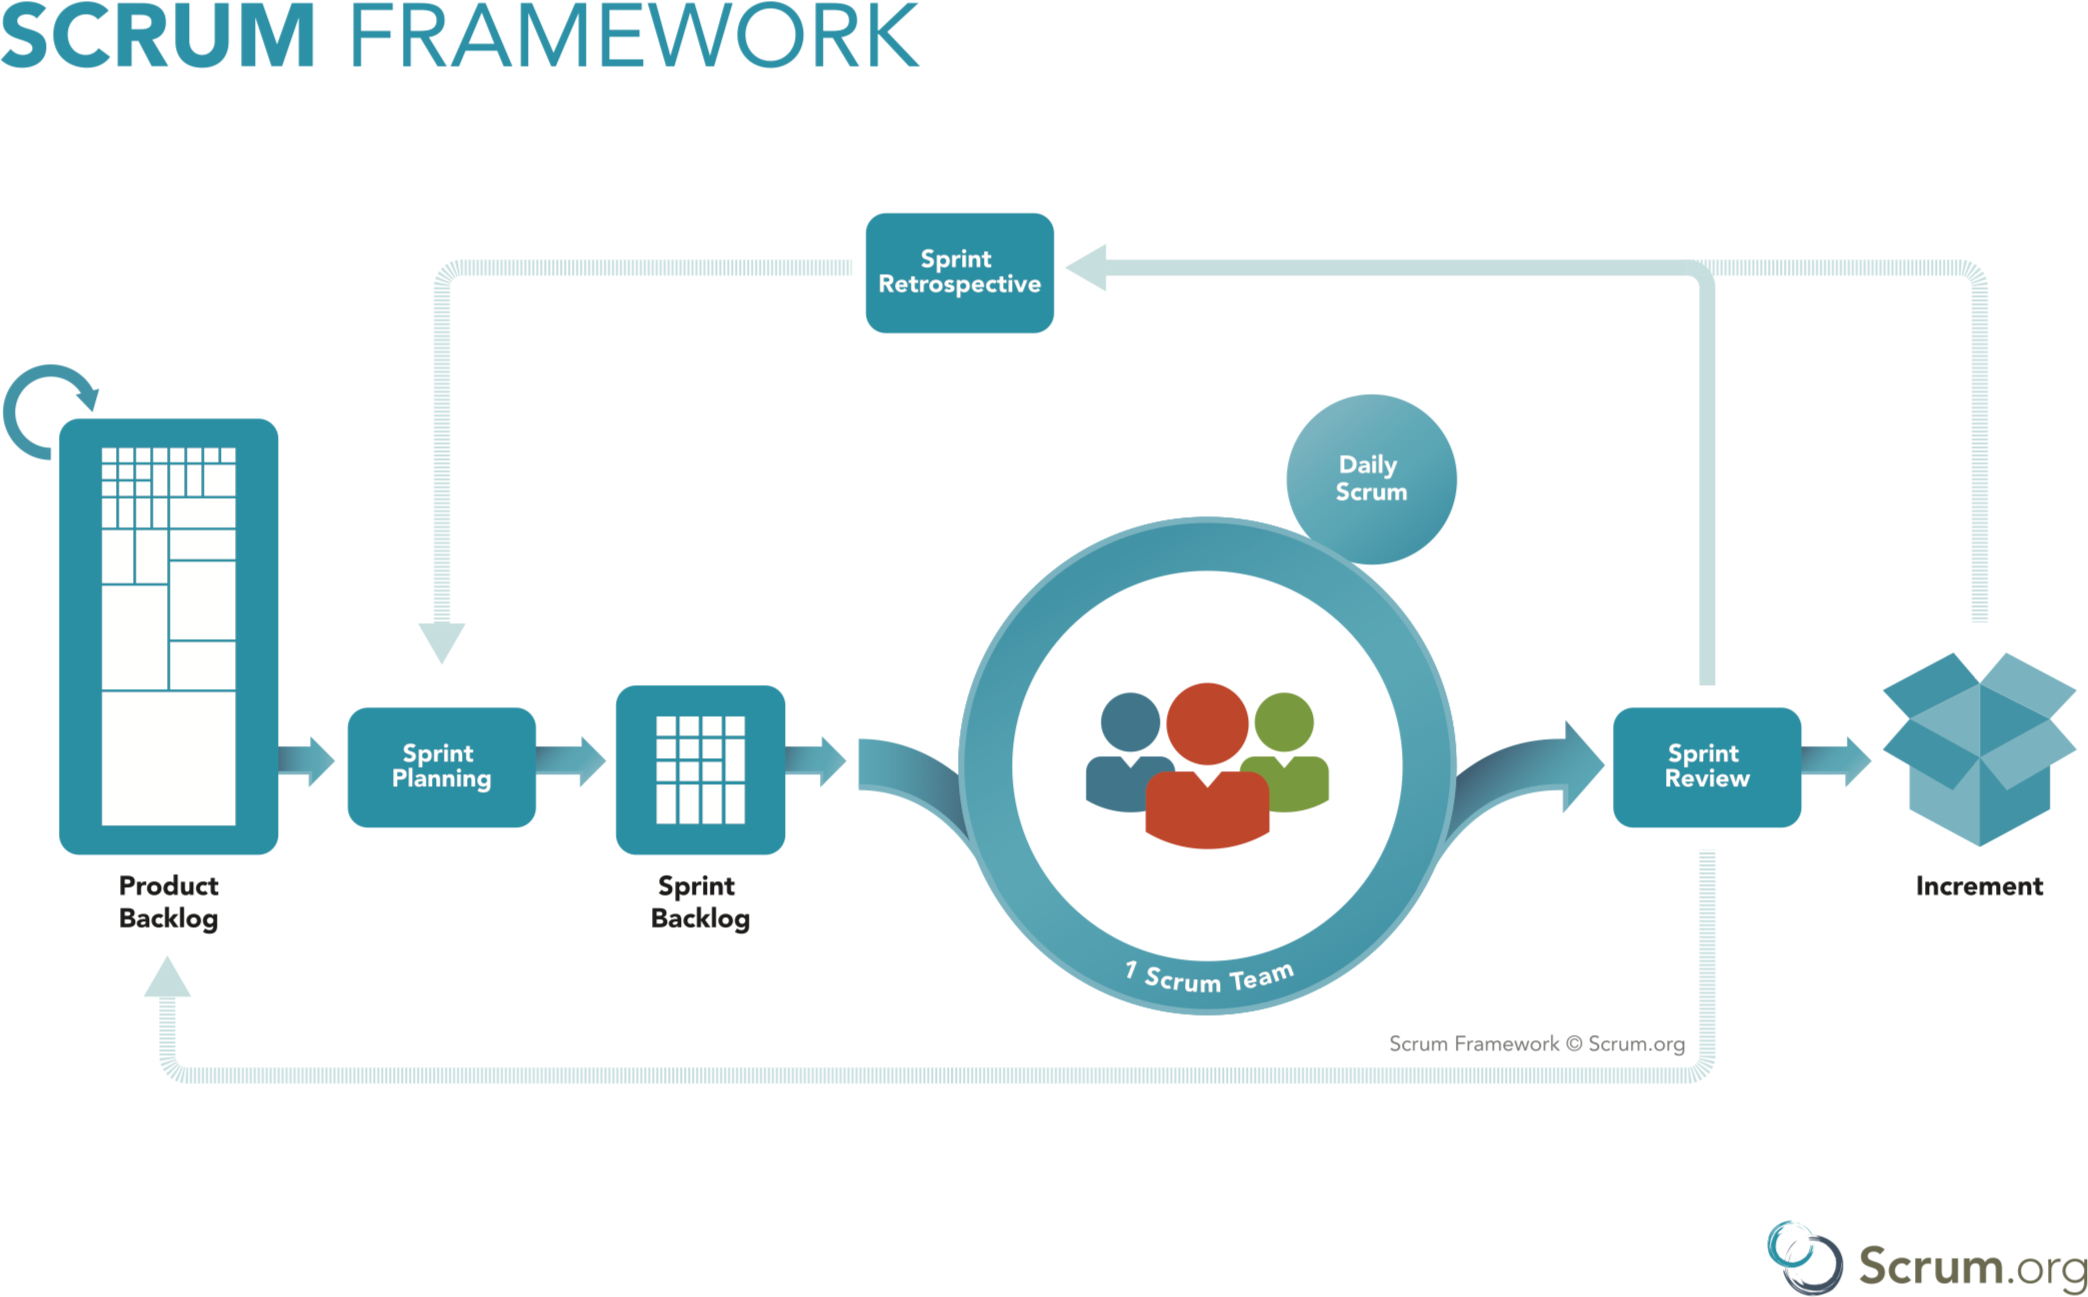
\includegraphics[width=0.9\textwidth]{img/scrum-framework.png}
    \caption[Scrum Framework]{Scrum Framework~\footcite{scrum_framework}}\label{fig:scrum_framework}
  \end{figure}
\end{savenotes}

Das Scrum Framework (Abbildung~\ref{fig:scrum_framework}) besteht aus drei Rollen, fünf Ereignissen und drei Artefakten.

\begin{itemize}
  \item \textbf{Rollen}
  \begin{itemize}
    \item \textbf{Development Team}: Selbstorganisiertes Team, das am Produkt arbeitet.
    \item \textbf{Scrum Master}: Verantwortlich dafür, sicherzustellen, dass Scrum verstanden und gelebt wird.
    \item \textbf{Product Owner}: Verantwortlich, den Wert des Produktes und die Arbeit des Development Teams zu maximieren.
  \end{itemize}
  \item \textbf{Ereignisse}
  \begin{itemize}
    \item \textbf{Sprint}: Ist das Herz von Scrum: eine Timebox von zwei bis vier Wochen, in dem ein fertiges, verwendbares und potentiell auslieferbares Produkt-Inkrement entwickelt wird.
    \item \textbf{Sprint Planning}: Planung eines Sprints. Hier verpflichtet sich das Scrum-Team, eine gewisse Anzahl an Aufgaben im kommenden Sprint abzuarbeiten.
    \item \textbf{Daily Scrum}: Tägliches, zeitlich begrenztes Meeting, bei dem von jedem Teammitglied folgende drei Fragen beantwortet werden:
    \begin{enumerate}
      \item Was habe ich gemacht?
      \item Was werde ich machen?
      \item Was behindert mich bei meiner Arbeit?
    \end{enumerate}
    \item \textbf{Sprint Review}: Abschluss eines Sprints. Hier präsentiert das Team dem Product Owner die Ergebnisse des letzten Sprints.
    \item \textbf{Sprint Retrospective}: Das Team reflektiert den Sprint-Ablauf und ergreift Maßnahmen, um den Prozess weiter zu verbessern.
  \end{itemize}
  \item \textbf{Artefakte}
  \begin{itemize}
    \item \textbf{Product Backlog}: Ist eine Sammlung von möglichen Aufgaben für das Team am Produkt. Sollte einen Ausblick auf die zukünftige Entwicklung des Produktes geben. Oben im Product Backlog befinden sich die bereits fein geplanten Aufgaben, weiter unten die groben.
    \item \textbf{Sprint Backlog}: Entspricht den Aufgaben, die vom Team in den Sprint genommen und dem Product Owner zugesagt wurden.
    \item \textbf{Inkrement}: Entsteht am Ende eines jeden Sprints und ist eine lauffähige Version des Produktes, die releasefähig ist.
  \end{itemize}
\end{itemize}

\subsection[Scrum in mehreren Teams]{Scrum in mehreren Teams~\footcite[vgl.][S.172ff]{scrum_kurz_gut_2013}}

Scrum beschreibt eine agile Vorgehensweise für ein Team (ein Team entwickelt ein Produkt).
In der Realität existieren aber oft mehrere Teams und/oder mehrere Produkte. 
Dahingehend muss die Organisation der unterschiedlichen Scrum-Teams individuell angepasst werden.
Für die Trennung der Teams gibt es unterschiedliche Ansätze:
\begin{description}
  \item[Trennung nach Organisationseinheiten] \hfill \\ Die Teams werden entlang der Abteilungsstruktur einer Organisation getrennt. Aus Scrum-Sicht macht das nicht immer Sinn, da bei der Umsetzung eines Features Abhängigkeiten zu anderen Teams bestehen (keine cross-funktionalen Teams).
  \item[Trennung nach Komponenten (Komponenten-Teams)] \hfill \\ Die technischen Komponenten werden den Teams zugeteilt, was ebenfalls zu Abhängigkeiten zu anderen Teams führt und eine gute Abstimmung zwischen den Teams voraussetzt.
  \item[Trennung nach fachlichen Themen (Feature-Teams)] \hfill \\ Jedes Team entwickelt, unabhängig von den anderen Teams, eine fachliche Komponente. Diese Variante erfüllt die Forderung des Scrum Frameworks nach cross-funktionalen Teams, weshalb bei dieser Form die Abstimmung zwischen den Teams am geringsten ist.
\end{description}

\begin{savenotes}
  \begin{figure}[H]
    \centering
    \subfigure[Feature-Teams]{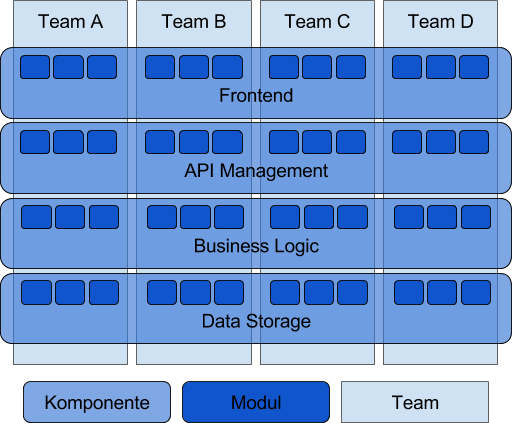
\includegraphics[width=0.40\textwidth]{img/feature-teams.png}} 
    \subfigure[Komponenten-Teams]{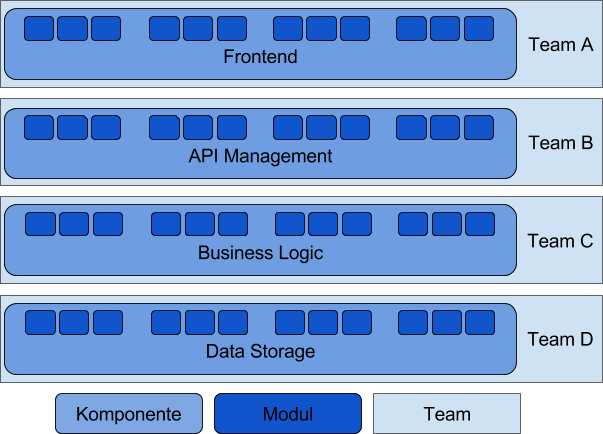
\includegraphics[width=0.48\textwidth]{img/component-teams.png}} 
  \caption{Scrum Teams}\label{fig:Scrum Teams}
  \end{figure}
\end{savenotes}

In allen Varianten existieren aber pro Team unterschiedliche Software-Module und (agile) Prozesse, die unabhängig voneinander die Team-Qualität als Gesamtes bestimmen.
\\
\\
Um Scrum auf mehrere Teams skalieren zu können, existieren bereits unterschiedlichste Frameworks.
Drei davon sind \ac{SoS}, \ac{LeSS} und Scrum at Scale, die im Folgenden kurz vorgestellt werden.

\clearpage
\subsubsection[\ac{SoS}]{\acf{SoS}~\footcite[vgl.][]{sos}}

\ac{SoS} ist eine Technik, um Scrum auf große Gruppen zu skalieren. 
Dabei werden die Gruppen in agile Teams von fünf bis zehn Personen geteilt.
Nach jedem Daily Scrum wird pro Team eine Botschafterin bestimmt, um an einem täglichen Meeting mit anderen Botschafterinnen teilzunehmen, das sogenannte Scrum of Scrums.
Je nach Kontext sind die Botschafterinnen technische Teilnehmer, Scrum Master oder sogar Team-Mana\-ger\-innen.
Das \ac{SoS} hat sein eigenes Backlog, bei dem es Fertigstellungen, nächste Schritte und Hindernisse im Auge behält.

\begin{savenotes}
  \begin{figure}[H] 
    \centering
       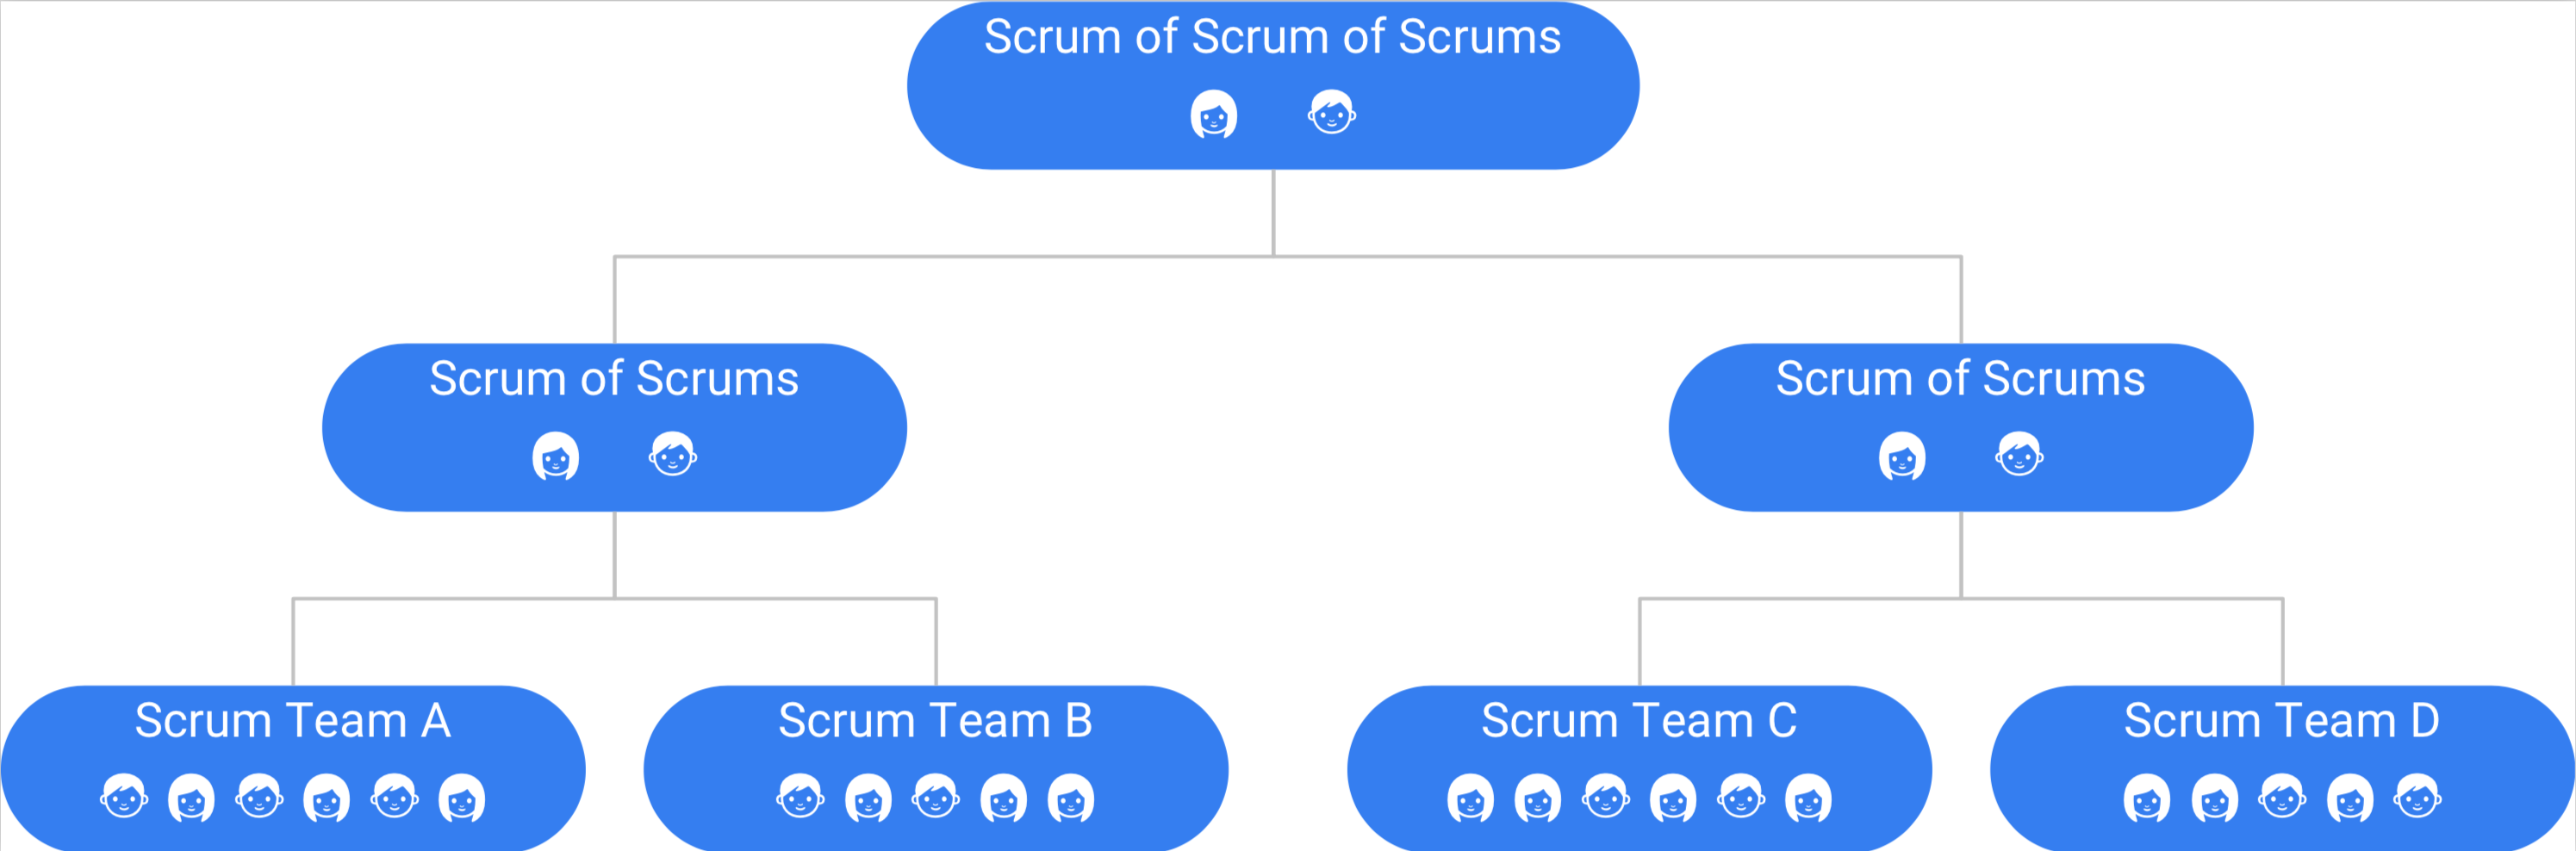
\includegraphics[width=1.0\textwidth]{img/sos.png}
    \caption{\ac{SoS} auf 3 Ebenen}\label{fig:sos}
  \end{figure}
\end{savenotes}

\ac{SoS} ist beliebig skalierbar, das ermöglicht auch mehrere Scrum of Scrums Ebenen, wie Abbildung~\ref{fig:sos} zeigt.

\subsubsection[\ac{LeSS}]{\acf{LeSS}~\footcite[vgl.][]{less}}

\ac{LeSS} adaptiert die Grundsätze von Scrum in einen größeren Rahmen.
Daher muss auch zuerst Scrum für ein Team verstanden werden, bevor mit \ac{LeSS} begonnen werden kann.
Es unterscheidet dabei zwei Varianten:
\begin{description}
  \item[LeSS] für bis zu 8 Teams mit jeweils acht Mitgliedern
  \item[LeSS Huge] bis zu mehrere tausend Personen an einem Produkt
\end{description}

\begin{savenotes}
  \begin{figure}[H] 
    \centering
       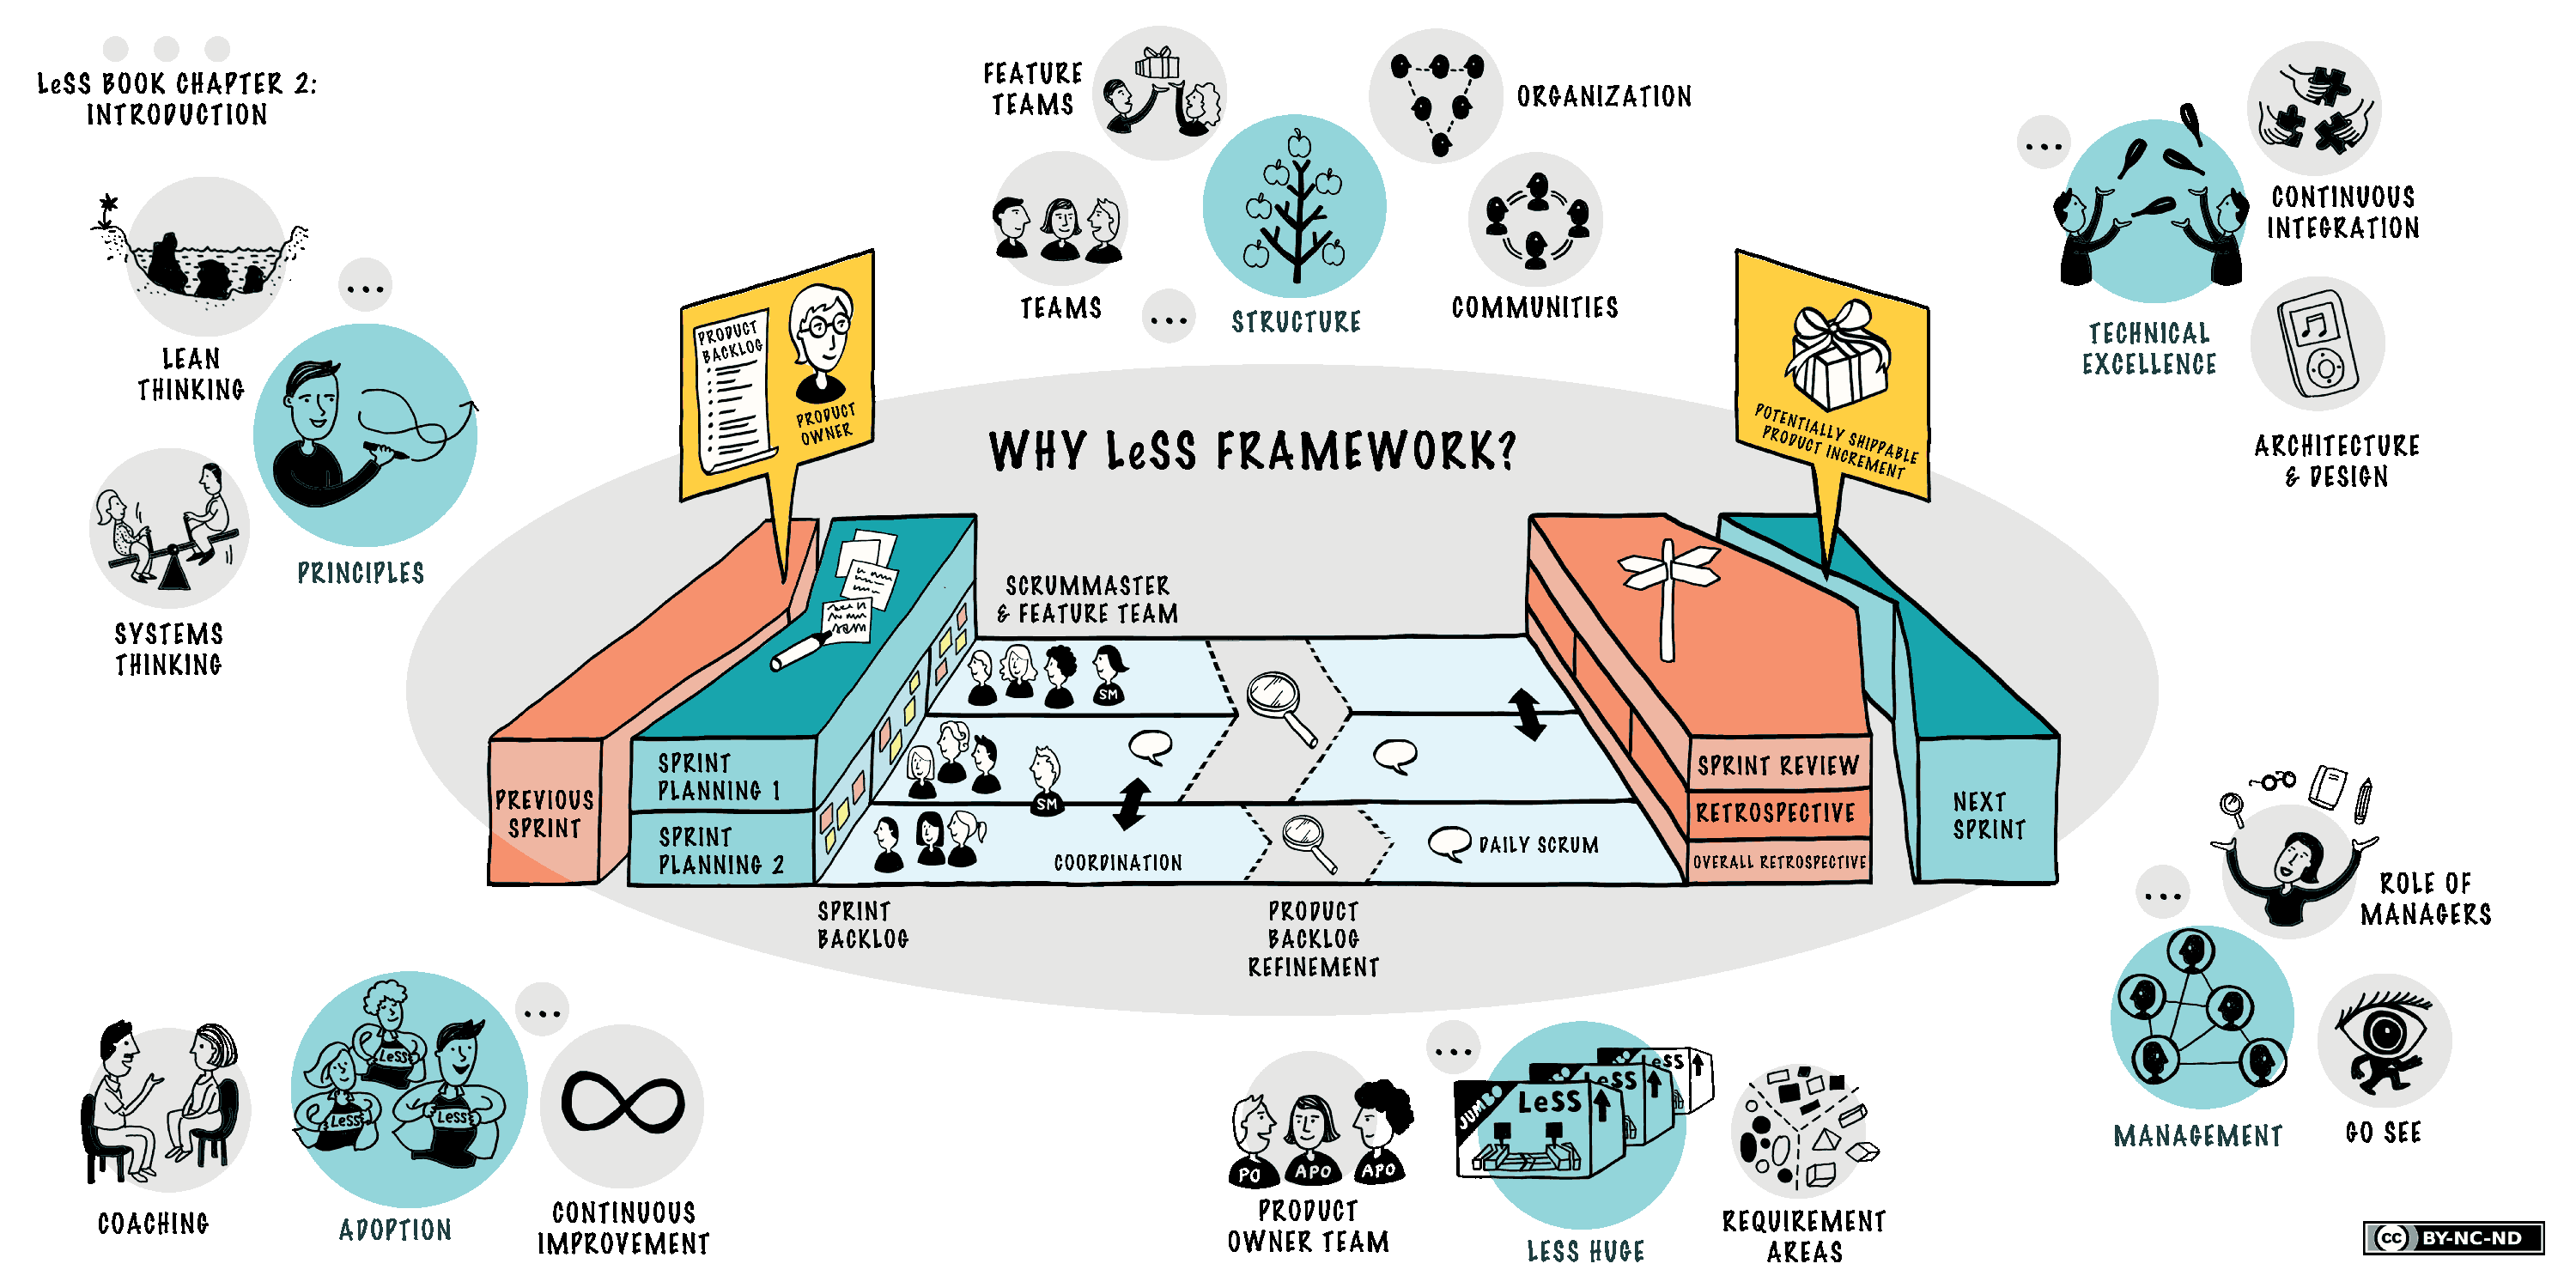
\includegraphics[width=1.0\textwidth]{img/less.png}
    \caption[\ac{LeSS} Framework]{\ac{LeSS} Framework~\footcite{less_framework}}\label{fig:less}
  \end{figure}
\end{savenotes}

Es gibt viele Dinge, die gleich bleiben, wie bei einem Team: Product Backlog, \ac{DoD}, nach jedem Sprint ein lauffähiges Inkrement, Product Owner, cross-funktionale Teams und ein Sprint.
Darüber hinaus gibt es aber auch einige Unterschiede:

\begin{description}
  \item[Sprint Planning 1] kann Personen von allen Teams beinhalten, die sich ihre Arbeit selbstständig aufteilen.
  \item[Sprint Planning 2] wird von jedem Team selbst abgehalten, es können aber mehrere Teams in einem Raum sein.
  \item[Daily Scrum] wird auch unabhängig in jedem Team abgehalten, aber eine Person aus Team A kann bei Team B dabei sein, um den Informationsfluss zu erhöhen.
  \item[Overall \ac{PBR}] ist kurz und informativ, um abzuklären, welches Team vermutlich welche Aufgabe übernimmt, für das spätere \ac{PBR}.
  \item[\ac{PBR}] können auch mehrere Teams gemeinsam machen, um voneinander zu lernen und besser koordinieren zu können.
  \item[Sprint Review] kann zusätzlich Personen aus anderen Teams oder andere Stakeholder beinhalten.
  \item[Overall Retrospective] ist ein ganz neues Meeting mit Scrum Mastern, Product Ownern und rotierenden Personen der Teams, um den Gesamtprozess zu verbessern.
\end{description}

\clearpage
\subsubsection[Scrum at Scale]{Scrum at Scale~\footcite[vgl.][]{scale}}

Scrum at Scale versucht Scrum skalierbar zu machen, durch ein Minimum an Bürokratie und eine frei skalierbare Architektur.
Es besteht aus Scrum Teams, die durch \ac{SoS} und Meta Scrums koordiniert werden. 
\begin{savenotes}
  \begin{figure}[H] 
    \centering
       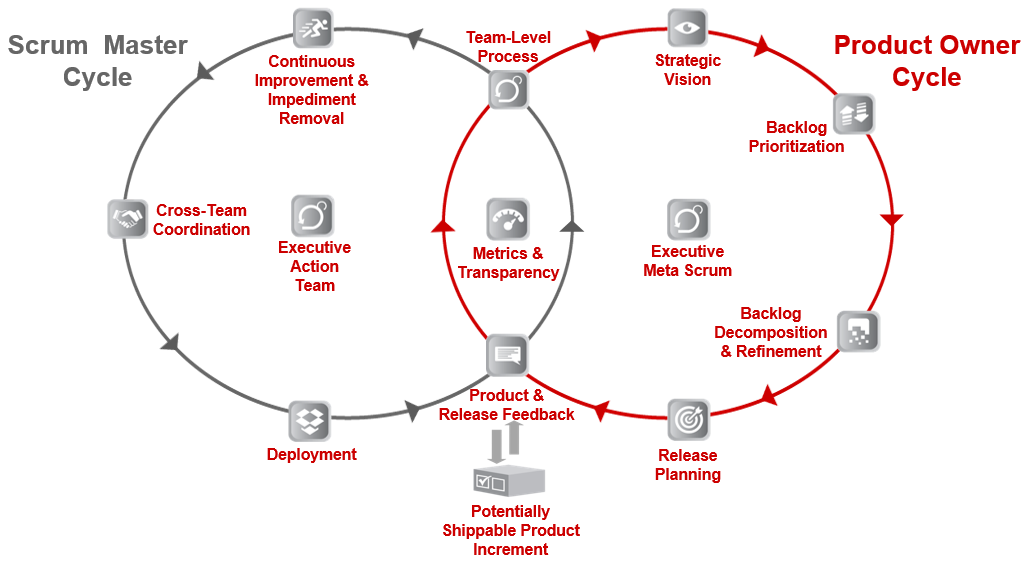
\includegraphics[width=1.0\textwidth]{img/scrumatscale.png}
    \caption[Scrum at Scale Framework {-} SMPO Zyklus]{Scrum at Scale Framework {-} SMPO Zyklus~\footcite{scrumatscale_framework}}\label{fig:sas}
  \end{figure}
\end{savenotes}

Das Was und das Wie werden bei Scrum at Scale durch zwei Zyklen getrennt, die sich nur an zwei Punkten schneiden (Abbildung~\ref{fig:sas}).
\begin{description}
  \item[Scrum Master Zyklus] \hfill \\ Wird über \ac{SoS} gesteuert und hat an der Spitze ein \ac{EAT}, welches die einzelnen \ac{SoS} koordiniert.
  \item[Product Owner Zyklus] \hfill \\ Ein Team von Product Ownern, die ein \ac{SoS} Backlog verantworten, nennt man Meta Scrum. Meta Scrums haben einen Chief Product Owner, der als Scrum Master agiert und verantwortlich für die Koordination der Product Backlogs ist. An der Spitze steht ein \ac{EMS}, der Visionen und strategische Ziele verfolgt.
\end{description}

Metriken und Transparenz im Allgemeinen werden bei Scrum at Scale groß geschrieben, da Scrum nur so optimal funktionieren kann.

\clearpage
\section[Software-Qualität]{Software-Qualität~\footcite[vgl.][Kapitel 1.2]{hoffmann_software_qualitat_2013}}

Eine mögliche Definition von Software-Qualität findet sich in der DIN-ISO-Norm 9126:

\begin{quote}
  ``Software-Qualität ist die Gesamtheit der Merkmale und Merkmalswerte eines Software-Produktes, die sich auf dessen Eignung beziehen, festgelegte Erfordernisse zu erfüllen.''
\end{quote}

Wie aus dieser Definition schon erkennbar ist, gibt es viele unterschiedliche Kriterien, um die Qualität von Software zu bewerten.
Einige wesentliche Merkmale, um die Qualität von Software bewerten zu können, lassen sich in kunden- und herstellerorientierte Merkmale unterteilen:

\begin{description}
  \item[Kundenorientierte Merkmale] \hfill \\ Nach außen hin sichtbare Merkmale, die sich auf den kurzfristigen Erfolg der Software auswirken, da sie die Kaufentscheidung möglicher Kunden beeinflussen.
  \begin{description}
    \item[Funktionalität (Functionality, Capability)] \hfill \\ Beschreibt die Umsetzung der funktionalen Anforderungen. Fehler sind hier häufig Implementierungsfehler (sogenannte Bugs), welche durch Qualitäts\-sich\-erung bereits in der Entwicklung entdeckt oder vermieden werden können. 
    \item[Laufzeit (Performance)] \hfill \\ Beschreibt die Umsetzung der Laufzeit-Anforderungen. Besonderes Augenmerk muss in Echtzeitsystemen auf dieses Merkmal gelegt werden.
    \item[Zuverlässigkeit (Reliability)] \hfill \\ Eine hohe Zuverlässigkeit ist in kritischen Bereichen, wie z.B. Medizintechnik oder Luftfahrt, unabdingbar. Erreicht werden kann diese aber nur durch die Optimierung einer Reihe anderer Kriterien.
    \item[Benutzbarkeit (Usability)] \hfill \\ Betrifft alle Eigenschaften eines Systems, die mit der Benutzerinnen-Interaktion in Berührung kommen.
  \end{description}
  \item[Herstellerorientierte Merkmale] \hfill \\ Sind die inneren Merkmale, die sich auf den langfristigen Erfolg der Software auswirken und somit als Investition in die Zukunft gesehen werden sollten.
  \begin{description}
    \item[Wartbarkeit (Maintainability)] \hfill \\ Die Fähigkeit, auch nach der Inbetriebnahme noch Änderungen an der Software vornehmen zu können. Wird oft vernachlässigt, ist aber essentiell für langlebige Software und ein großer Vorteil gegenüber der Konkurrenz.
    \item[Transparenz (Transparency)] \hfill \\ Beschreibt, wie die nach außen hin sichtbare Funktionalität intern umgesetzt wurde. Gerade bei alternder Software kann es zu einer Unordnung kommen, welche auch Software-Entropie (Grad der Unordnung) genannt wird.
    \item[Übertragbarkeit] \hfill \\ Wird auch Portierbarkeit genannt und beschreibt die Eigenschaft einer Software, in andere Umgebungen übertragen werden zu können (zum Beispiel 32-Bit zu 64-Bit oder Desktop zu Mobile).
    \item[Testbarkeit (Testability)] \hfill \\ Testen stellt eine große Herausforderung dar, da oft auf interne Zustände zugegriffen werden muss oder die Komplexität durch die möglichen Eingangskombinationen vervielfacht wird. Aber gerade durch Tests können Fehler frühzeitig entdeckt und behoben werden.
  \end{description}
\end{description}

Je nach Anwendungsgebiet und Anforderungen an die Software haben die Merkmale unterschiedliche Relevanz und einige können sich auch gegenseitig beeinflussen, wie aus der Korrelationsmatrix in Abbildung~\ref{fig:korrelationsmatrix} ersichtlich.
Dabei sind die positiv korrelierenden Merkmale mit einem Plus und die negativ korrelierenden mit einem Minus gekennzeichnet.

\begin{savenotes}
  \begin{figure}[H] 
    \centering
       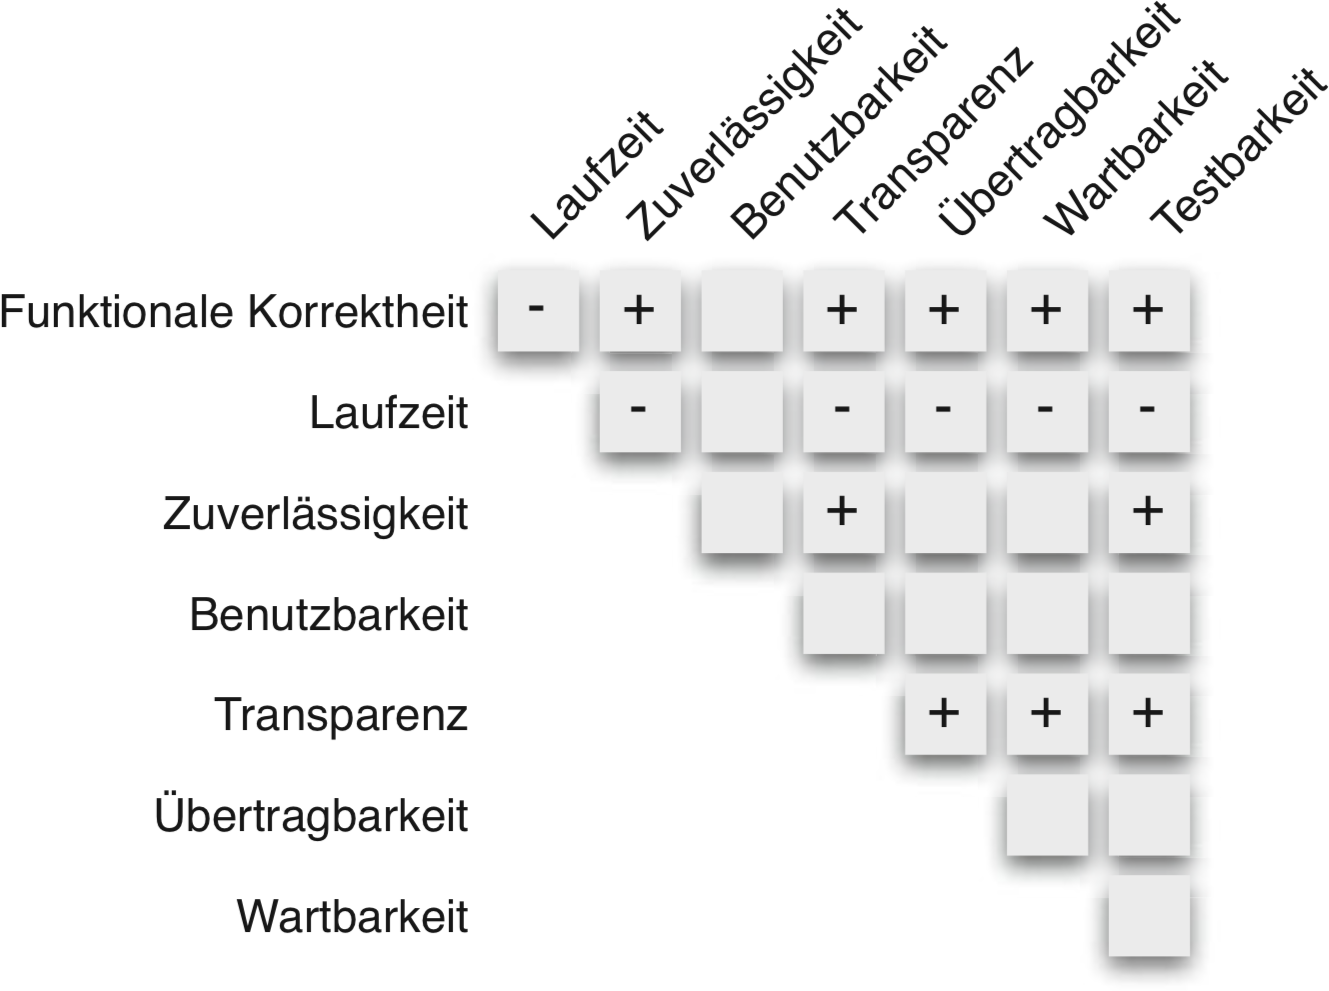
\includegraphics[width=0.6\textwidth]{img/korrelationsmatrix-kriterien.png}
    \caption[Korrelationsmatrix Qualitätskriterien]{Korrelationsmatrix Qualitätskriterien~\footcite[][S. 11, Abb. 1.3]{hoffmann_software_qualitat_2013}}\label{fig:korrelationsmatrix}
  \end{figure}
\end{savenotes}

\begin{savenotes}
  \begin{figure}[H] 
    \centering
       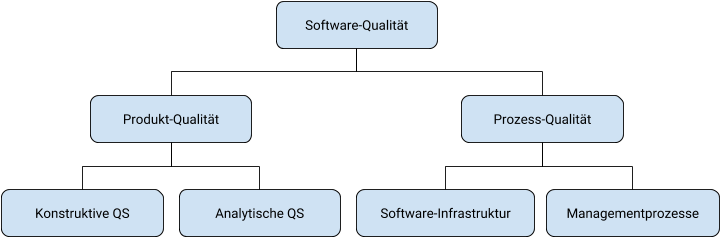
\includegraphics[width=1.0\textwidth]{img/software-quality.png}
    \caption[Software-Qualität]{Software-Qualität}\label{fig:software-quality}
  \end{figure}
\end{savenotes}

Um die oben genannten Merkmale verbessern zu können, lassen sich die Techniken und Methoden zur Qualitätssicherung, wie in Abbildung~\ref{fig:software-quality} ersichtlich, in die Bereiche Produkt- und Prozessqualität einteilen, welche im Folgenden noch genauer beschrieben werden.

\subsection[Produktqualität]{Produktqualität~\footcite[vgl.][Kapitel 1.4.1]{hoffmann_software_qualitat_2013}}

Die Produktqualität lässt sich in die zwei Bereiche konstruktive und analytische Qualitätssicherung unterteilen.
Während die konstruktive Qualitätssicherung sich mit den Vorgaben beschäftigt, die ein Softwareprodukt im Vorhinein (während der Entwicklung) erfüllen muss, dient die analytische Qualitätssicherung dem Analysieren und Bewerten im Nachhinein (des fertigen Produktes).

\begin{description}
  \item[Konstruktive Qualitätssicherung] \hfill
  \begin{description}
    \item[Software-Richtlinien] \hfill \\ Eine solche Richtlinie gibt Regeln vor, wie Konstrukte einer Sprache zu verwenden sind. Können unternehmensspezifisch sein, aber auch allgemeinen Standards folgen.
    \item[Typisierung] \hfill \\ Typisierte Sprachen können Inkonsistenzen bereits frühzeitig erkennbar machen.
    \item[Vertragsbasierte Programmierung] \hfill \\ Basiert auf einer gezielten Angabe von Bedingungen (Vor-, Nachbedingungen, Invarianten, Zusicherungen) für Funktionen und Prozeduren, sogenannten Verträgen.
    \item[Fehlertolerante Programmierung] \hfill \\ Fehler in der Software können nie ganz vermieden werden, aber es kann intelligent auf mögliche Fehler reagiert werden.
    \item[Portabilität] \hfill \\ Portabler Programmcode ist oft allgemeiner gehalten und kann auch die Transparenz (und somit die Fehlerdichte) positiv beeinflussen.
    \item[Dokumentation] \hfill \\ Enthält die Erstellung von Standards und das Dokumentieren selbst.
  \end{description}
  \item[Analytische Qualitätssicherung] \hfill
  \begin{description}
    \item[Software-Test] \hfill \\ Testen des Software-Produktes mit vordefinierten Tests. Die Auswahl dieser Tests beeinflusst dabei direkt die Qualität. Es wird zwischen Black-Box- und White-Box-Tests unterschieden und es können Testmetriken verwendet werden, um die Qualität der Tests zu bestimmen.
    \item[Statische Analyse] \hfill \\ Hier wird im Gegensatz zu den Software-Tests das Programm nicht ausgeführt, sondern es wird direkt der Quelltext analysiert. Es gibt folgende Möglichkeiten der statischen Analyse:
    \begin{description}
      \item[Software-Metriken] \hfill 
      \item[Konformitätsanalyse] \hfill 
      \item[Exploit-Analyse] \hfill 
      \item[Anomalienanalyse] \hfill 
      \item[Manuelle Software-Prüfung] \hfill 
    \end{description}
    \item[Software-Verifikation] \hfill \\ Es wird versucht, gewisse Eigenschaften des Programms formal auf mathematischem Wege zu beweisen.
  \end{description}
\end{description}

\subsection[Prozessqualität]{Prozessqualität~\footcite[vgl.][Kapitel 1.4.2]{hoffmann_software_qualitat_2013}}

Die Prozessqualität beschäftigt sich im Gegensatz zur Produktqualität mit der Entstehung des Software-Produktes, genauer genommen mit dem Prozess dahinter.
Dieser Prozess kann in eine Entwicklerinnensicht, mit der Software-Infrastruktur, und eine Managementsicht, mit den Managementprozessen, aufgeteilt werden.

\begin{description}
  \item[Software Infrastruktur] \hfill \\ Unterstützt die Entwicklerin bei der täglichen Arbeit.
  \begin{description}
    \item[Konfigurationsmanagement] \hfill \\ Hilft bei der Verwaltung der entstehenden Artefakte, zum Beispiel durch den Einsatz von \ac{VCS}.
    \item[Build-Automatisierung] \hfill \\ Erzeugt die Artefakte voll automatisch.
    \item[Test-Automatisierung] \hfill \\ Genauso, wie das Erstellen der Artefakte, wird auch das Testen vollautomatisch durchgeführt.
    \item[Defektmanagement] \hfill \\ Um Defekte zentral erfassen und verwalten zu können.
  \end{description}
  \item[Managementprozesse] \hfill \\ Steuern den Projektablauf und werden in Vorgehensmodelle und Reifegradmodelle unterteilt.
  \begin{description}
    \item[Vorgehensmodelle] \hfill \\ Regeln die grundlegenden Arbeitsabläufe in einem Projekt, zum Beispiel über das V-Modell oder Scrum.
    \item[Reifegradmodelle] \hfill \\ Haben das Ziel, Prozesse zu analysieren und zu optimieren.
  \end{description}
\end{description}

\clearpage
\section{Metriken}

Eine Softwaremetrik wird vom \ac{IEEE} Standard 1061 von 1998 folgendermaßen definiert:
\begin{quote}
  ``Eine Softwarequalitätsmetrik ist eine Funktion, die eine Software-Einheit in einen Zahlenwert abbildet, welcher als Erfüllungsgrad einer Qualitätseigenschaft der Software-Einheit interpretierbar ist.''\footcite[vgl.][S.3]{ieee-1061}
\end{quote}

Vereinfacht gesagt, ist eine Metrik eine oder mehrere Kennzahlen, die mithilfe einer Funktion ein Qualitätsmerkmal in einen Zahlenwert abbildet.
Eine Kennzahl kann daher auch schon direkt eine Metrik sein, wenn sie in der Lage ist, ein gewünschtes Qualitätsmerkmal abzubilden.

\begin{savenotes}
  \begin{figure}[H] 
    \centering
       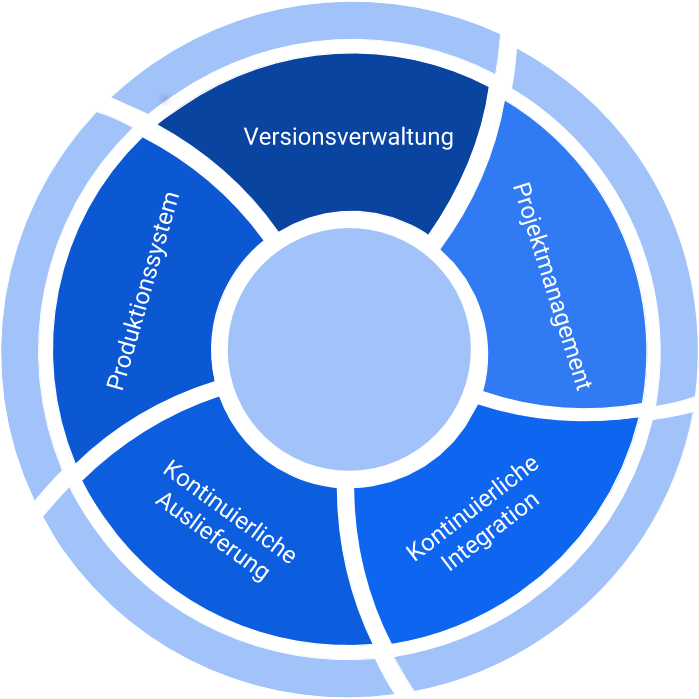
\includegraphics[width=0.6\textwidth]{img/software-development-lifecycle.png}
    \caption[Systeme im Softwareentwicklungsprozess]{Systeme im Softwareentwicklungsprozess~\label{fig:sdlc}}
  \end{figure}
\end{savenotes}

Im Entwicklungsprozess werden in den unterschiedlichen Systemen und Prozessschritten Daten erzeugt, die als Kennzahlen oder direkt als Metriken genutzt werden können.
Abbildung~\ref{fig:sdlc} zeigt die einzelnen Schritte und Systeme im Entwicklungsprozess.~\footcite[vgl.][S.8]{davis_agile_2015}

\subsection[Versionsverwaltung]{Versionsverwaltung~\footcite[vgl.][S.62ff]{davis_agile_2015}}

Das \acf{VCS} befindet sich nah an der Arbeit der Entwicklerinnen, da hier der Quellcode des Produktes verwaltet wird.
Daher können hier Daten darüber gesammelt werden, wie viel gearbeitet und auch wie viel zusammengearbeitet wird.
Um bestmögliche Daten zu bekommen, sollten verteilte Versionskontrollsysteme wie Git verwendet und mit Pull Requests gearbeitet werden.

\begin{description}
  \item[\ac{CLOC}] \hfill \\ Anzahl der geänderten Codezeilen.
  \item[\ac{CLOC} pro Entwicklerin] \hfill \\ Anzahl der geänderten Zeilen im Quellcode pro Entwicklerin.
  \item[Commits] \hfill \\ Gesamtzahl an Commits in einem bestimmten Zeitraum.
  \begin{description}
    \item[Commits pro Entwicklerin] \hfill \\ Gesamtzahl an Commits in einem bestimmten Zeitraum pro Entwicklerin.
    \item[Kommentare pro Commit] \hfill \\ Anzahl der Kommentare pro Commit.
    \item[\ac{CLOC} pro Commit] \hfill \\ Anzahl der geänderten Zeilen im Quellcode pro Commit.
  \end{description}
  \item[Pull Requests] \hfill \\ Gesamtzahl an Pull Requests in einem bestimmten Zeitraum.
  \begin{description}
    \item[Gemergte Pull Requests] \hfill \\ Anzahl erfolgreicher Pull Requests in einem bestimmten Zeitraum.
    \item[Abgelehnte Pull Requests] \hfill \\ Anzahl abgelehnter Pull Requests in einem bestimmten Zeitraum.
    \item[Kommentare pro Pull Request] \hfill \\ Anzahl der Kommentare pro Pull Request.
  \end{description}
\end{description}

\subsection[Projektmanagement]{Projektmanagement~\footcite[vgl.][S.37ff]{davis_agile_2015}}

In einem \acf{PTS}, oft auch Issue Tracker oder Issue Tracking System genannt, werden Aufgaben definiert und zugewiesen, Bugs verwaltet und Arbeitszeit mit Aufgaben verknüpft.
Hier können Daten über das Projektverständnis des Teams, die Geschwindigkeit und vor allem die Konsistenz der Arbeit gesammelt werden.
Um bestmögliche Daten erhalten zu können, gibt es folgende Empfehlungen:
\begin{itemize}[noitemsep]
  \item \ac{PTS} wird von allen genutzt
  \item Aufgaben mit möglichst vielen Tags versehen
  \begin{itemize}
    \item Aufgaben kategorisieren (nach ``gut'', ``ok'' und ``schlecht'')
  \end{itemize}
  \item Aufgaben schätzen
  \item gemeinsam eine \ac{DoD} festlegen
\end{itemize}
Jede Arbeit, die am \ac{PTS} vorbei geht, fällt später bei der Auswertung der Daten durch das Raster.
Durch das Kategorisieren der Aufgaben können später Korrelationen ausgewertet werden, vor allem auch durch das Zuweisen von Tags wird sichtbar, wie gut die Aufgabe abgelaufen ist.
Zusätzlich kann durch die geschätzte und tatsächliche Arbeitszeit eine qualitative Aussage über die Schätzungen des Teams getroffen werden.
Eine \ac{DoD} hilft allgemein den Prozess zu verbessern und Rückläufe im Arbeitsablauf zu minimieren.

Dadurch ergeben sich folgende Kennzahlen aus einem \ac{PTS}:
\begin{description}
  \item[Burn Down] \hfill \\ Die Anzahl erledigter Arbeit über die Zeit. Liefert einen Richtwert, wo man sich gerade im Sprint befindet, verglichen zum optimalen Verlauf.
  \item[Velocity] \hfill \\ Eine relative Messung der Konsistenz erledigter Arbeit über die Sprints.
  \item[Cumulative Flow] \hfill \\ Zeigt, wie viel Aufgaben nach Status dem Team zugewiesen sind, über die Zeit.
  \item[Lead Time] \hfill \\ Zeit zwischen Start und Abschluss einer Aufgabe, vor allem interessant bei Kanban.
  \item[Bug Counts] \hfill \\ Die Anzahl an Bugs über die Zeit.
  \begin{description}
    \item[Bug-Erzeugungsrate] \hfill \\ Anzahl Bugs nach Erstellungsdatum.
    \item[Bug-Fertigstellungsrate] \hfill \\ Anzahl Bugs nach Erledigungsdatum.
  \end{description}
  \item[Aufgaben-Volumen] \hfill \\ Die Anzahl der Aufgaben. Kann der Schätzung gegenübergestellt werden, um die Größe der Aufgaben oder ungeplante Arbeit aufzuzeigen.
  \item[Aufgaben-Rückfälligkeit] \hfill \\ Zeigt auf, wie oft Aufgaben im Arbeitsablauf rückwärts gehen.
\end{description}

\subsection[Kontinuierliche Integration und Auslieferung]{Kontinuierliche Integration und Auslieferung~\footcite[vgl.][S.84ff]{davis_agile_2015}}

\acf{CI}- und \acf{CD}-Systeme stellen sicher, dass die erstellte Software zu jedem Zeitpunkt auslieferbar ist, in dem sie zu definierten Zeitpunkten automatisch neu gebaut und ausgeliefert wird.
In einer solchen Build-Pipeline können sehr viel nützliche Daten erzeugt werden, vor allem mit Tools für statische Analysen (wie zum Beispiel SonarQube~\footcite[][]{sonarqube}).
Diese Systeme sind aber auch jene Elemente im Softwareentwicklungsprozess, die von Team zu Team am meisten variieren können.
Daher hängen die erzeugten Daten auch stark vom jeweiligen Setup ab.
Grundsätzlich können aber folgende Kennzahlen aus diesen Systemen ermittelt werden:

\begin{description}
  \item[Build-Dauer] \hfill \\ Geschätzte und tatsächliche Dauer der Builds.
  \item[Build-Status] \hfill \\ Es können die Anzahl der erfolgreichen und fehlerhaften Builds gegenübergestellt werden.
  \item[Build-Frequenz] \hfill \\ Wie oft wird ein Build ausgelöst.
  \item[Test Reports] \hfill \\ Anzahl erfolgreicher und fehlerhafter Tests, Gesamtdauer der Tests.
  \item[Code Coverage] \hfill \\ Wie viel Prozent des Quellcodes ist mit Tests abgedeckt.
  \item[Stresstests oder Benchmarking] \hfill \\ Wird oft im Build-Prozess getestet mit Tools wie JMeter~\footcite[][]{jmeter} oder Gatling~\footcite[][]{gatling}.
\end{description}

\subsection[Produktionssystem]{Produktionssystem~\footcite[vgl.][S.107ff]{davis_agile_2015}}

Daten aus den Produktionssystemen können gesammelte \acf{APM}- oder auch \acf{BI}-Kennzahlen sein.
Diese Kennzahlen ermöglichen Aussagen, ob die Kunden zufrieden sind und wie das System arbeitet.
Die \ac{BI}-Kennzahlen sollten möglichst nahe am Entwicklungsteam gehalten werden, damit es verstehen kann, wie die Kunden die Applikation nutzen.
Dazu können Frameworks wie StatsD~\footcite[][]{statsd} und Atlas~\footcite[][]{atlas} verwendet werden.
Im Produktionssystem können folgende Kennzahlen ermittelt werden:

\begin{description}
  \item[CPU Nutzung] \hfill \\ Auslastung der Prozessoren über die Zeit.
  \item[Heap Size] \hfill \\ Auslastung des Heap über die Zeit.
  \item[Fehlerraten] \hfill \\ Anzahl Fehler über die Zeit (kann aus dem Logging kommen).
  \item[Antwortzeiten] \hfill \\ Dauer der Verarbeitung bestimmter Anfragen.
  \item[Benutzerinnenanzahl] \hfill \\ Anzahl gleichzeitiger Benutzerinnen in der Applikation über die Zeit.
  \item[Aufenthaltsdauer] \hfill \\ Verweildauer der Benutzerinnen auf bestimmten Seiten.
  \item[Conversion Rate] \hfill \\ Anzahl Benutzerinnen, die zu Kunden wurden.
  \item[Semantisches Logging] \hfill \\ Ermöglicht es, beim Logging strukturierte Daten auszugeben, zum Beispiel: was suchen Benutzerinnen auf bestimmten Seiten.
  \item[Verfügbarkeit] \hfill \\ Verfügbarkeit der Applikation über die Zeit.
\end{description}

\subsection{Übersicht Kennzahlen im Entwicklungsprozess}

Die Metriken finden sich nochmal als Tabelle dargestellt und mit den dazugehörigen Fragen, die sie jeweils beantworten, im Anhang~\ref{appendix:metrics}.

\subsection[Eigene Metriken erstellen]{Eigene Metriken erstellen~\footcite[vgl.][S.127ff]{davis_agile_2015}}

Um eigene Metriken erstellen zu können, sind zwei Dinge notwendig:
\begin{itemize}
  \item Daten
  \item eine Funktion, um die Metrik zu berechnen
\end{itemize}

Dabei sollte darauf geachtet werden,
\begin{itemize}
  \item dass man auf die Metrik reagieren kann (Dinge, die einen stören und die man nicht ändern kann, frustrieren oder demotivieren)
  \item dass sich die Metrik nach den Team-Grundsätzen und Kerngeschäften ausrichtet, also nur Metriken, die einen bestimmten Zweck erfüllen und einem Ziel folgen
  \item dass die Metrik für sich alleine stehen kann
\end{itemize}

\subsection[Veröffentlichung von Metriken]{Veröffentlichung von Metriken~\footcite[vgl.][S.177ff]{davis_agile_2015}}

Metriken können auf verschiedene Art und Weise veröffentlicht werden. Zwei mögliche Beispiele sind Dashboards oder E-Mails.
Grundsätzlich sollte beachtet werden, dass man sich bei der Veröffentlichung von Metriken innerhalb der Grenzen und Gewohnheiten des Unternehmens bewegen sollte.
Außerdem sollte auf folgende Punkte geachtet werden:

\begin{description}
  \item[Dashboards] \hfill
  \begin{itemize}[noitemsep]
    \item den Zugriff innerhalb der Firma nicht einschränken
    \begin{itemize}[noitemsep]
      \item aber als intern ansehen
    \end{itemize}
    \item muss nach den Bedürfnissen der Teams anpassbar sein
    \item Metriken werden als Werkzeug gesehen, nicht als Waffe (gegen andere Teams oder Personen)
    \item Page Tracking verwenden, um das Nutzungsverhalten zu verstehen
  \end{itemize}
  \item[E-Mails] \hfill
  \begin{itemize}[noitemsep]
    \item aus dem Dashboard als Option wählbar machen (sonst landen sie schnell automatisch im Spam-Ordner)
    \item minimal erforderliche Daten, den Rest verlinken zum Dashboard
    \item den richtigen Rhythmus finden (zwischen oft genug informieren und nerven)
  \end{itemize}
\end{description}

Arbeitet ein Unternehmen beispielsweise viel mit Reports via E-Mail, dann kann ein reines Dashboard weniger Anerkennung finden. Hier könnte beispielsweise eine Übersicht per Mail versendet und mit Links zum Dashboard versehen werden.

\subsection[Agile Prinzipien messen]{Agile Prinzipien messen~\footcite[vgl.][S.201ff]{davis_agile_2015}}

Um die agilen Prinzipien messen zu können, muss zuerst herausgefunden werden, was die Kernaussagen dieser Prinzipien sind.
Dies kann zum Beispiel grafisch durch die Erstellung einer Wortwolke, wie in Abbildung~\ref{fig:wordcloud_principles} ersichtlich, erreicht werden.

\begin{savenotes}
  \begin{figure}[H] 
    \centering
    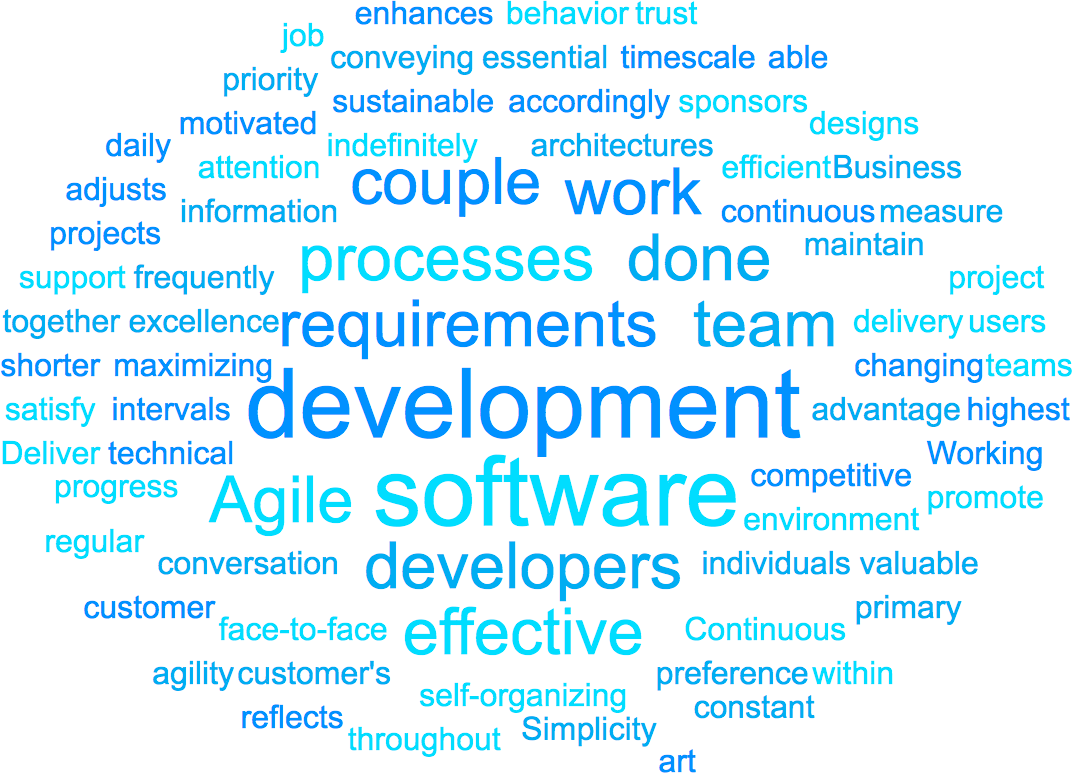
\includegraphics[width=0.9\textwidth]{img/principles-wordcloud.png}
    \caption{Agile Prinzipien als Wortwolke}\label{fig:wordcloud_principles}
  \end{figure}
\end{savenotes}

Aus dieser Wortwolke heben sich neben den Begriffen ``development'' und ``software'' vor allem auch die Begriffe ``team'', ``processes'', ``effective'' und ``requirements'' hervor.
Mithilfe dieser Begriffe lassen sich folgende vier Punkte ableiten:

\begin{itemize}[noitemsep]
  \item Effektive Software
  \item Effektiver Prozess
  \item Effektives Team 
  \item Effektive Anforderungen 
\end{itemize}

Für jeden dieser vier Punkte sind Metriken aus den unterschiedlichsten Systemen anwendbar~\footcite[vgl.][S.219ff]{davis_agile_2015}:

\begin{description}
  \item[Effektive Software] \hfill
  \begin{itemize}[noitemsep]
    \item erfolgreiche / fehlerhafte Builds
    \item Business-Metriken
    \item Status der Applikation
    \begin{itemize}[noitemsep]
      \item Fehlerraten
      \item CPU- / Speicherauslastung
      \item Antwort- / Transaktionszeiten
      \item Heap Größe / Garbage Collection / Anzahl Threads
    \end{itemize}
  \end{itemize}
  \item[Effektiver Prozess] \hfill
  \begin{itemize}[noitemsep]
    \item Velocity
    \item \ac{PTS} und \ac{VCS} Kommentare
    \item erfolgreiche Releases
  \end{itemize}
  \item[Effektives Team] \hfill
  \begin{itemize}[noitemsep]
    \item Lead Time
    \item \ac{MTTR}
    \item Deploy-Frequenz
    \item fehlerhafte Builds
  \end{itemize}
  \item[Effektive Anforderungen] \hfill
  \begin{itemize}[noitemsep]
    \item Rückläufigkeit
    \item Lead Time
    \item \ac{MTTR}
    \item Velocity
  \end{itemize}
\end{description}

\clearpage
\section[Qualitätsmodelle]{Qualitätsmodelle~\footcite[vgl.][S.29ff]{wagner_software_2013}}

Qualitätsmodelle sind das Fundament für Software-Produkt-Qualitätskontrolle und werden genutzt, um Qualität zu beschreiben, zu schätzen und/oder vorherzusagen.
Es wurden in den letzten Jahrzehnten unzählige Modelle vorgestellt.
Diese lassen sich in drei Kategorien einteilen: hierarchische, metamodellbasierte und implizite Modelle.

\begin{description}
  \item[Hierarchische Qualitätsmodelle] \hfill \\ Entstanden bereits in den 1970er Jahren. Qualität wird hierarchisch in Qualitätsfaktoren zerlegt, wie Wartbarkeit oder Zuverlässigkeit. Die Idee dahinter ist, Qualität hierarchisch herunterzubrechen, damit sie messbar wird. Verschiedenste Kritiken heben hervor, dass die Prinzipien zur Dekomposition von Qualitäts-Charakteristiken oft mehrdeutig sind. Außerdem sind die resultierenden Qualitäts-Charakteristiken nicht spezifisch genug, um direkt gemessen werden zu können.
  \item[Metamodellbasierte Qualitätsmodelle] \hfill \\ Entstanden in den 1990er Jahren, als Forscher ausgereiftere Wege aufzeigten, um Qualitäts-Charakteristiken zu zerlegen. Dadurch entstanden auch ausführlichere Metamodelle. Ein Metamodell beschreibt, wie gültig Qualitätsmodelle strukturiert sind. Die vielen Metamodelle zeigen, dass Qualität mehr Struktur in Qualitätsmodellen, als in abstrakten Qualitäts-Charakteristiken und Metriken braucht. Es wurde kein generelles Basis-Qualitätsmodell eingeführt, das man herunterladen und anwenden kann.
  \item[Statistische und implizite Qualitätsmodelle] \hfill \\ Für unterschiedlichste Qualitätsfaktoren wurden statistische Modelle vorgestellt, die Eigenschaften erfassen und Qualitätsfaktoren schätzen oder voraussagen. Auch Qualitäts-Analysetools nutzen eine Art Qualitätsmodell und auch Checklisten in der Entwicklung oder in Reviews sind eine Art Qualitätsmodell.
\end{description}

\subsection[\ac{FCM}-Modell]{\acf{FCM}-Modell~\footcite[vgl.][S.668ff]{abts_masterkurs_2009}}

Beim \ac{FCM}-Qualitätsmodell, welches zu den hierarchischen Qualitätsmodellen gehört, werden zunächst die erforderlichen Qualitätsmerkmale über die Anforderungen an die Software ermittelt.
In einem weiteren Schritt werden die Qualitätsmerkmale in kleinere Teilmerkmale aufgeteilt.
Dieser Schritt kann über mehrere Ebenen weitergeführt werden, bis es möglich ist, das Teilmerkmal direkt über eine oder mehrere Metriken abzubilden.

\begin{savenotes}
  \begin{figure}[H] 
    \centering
    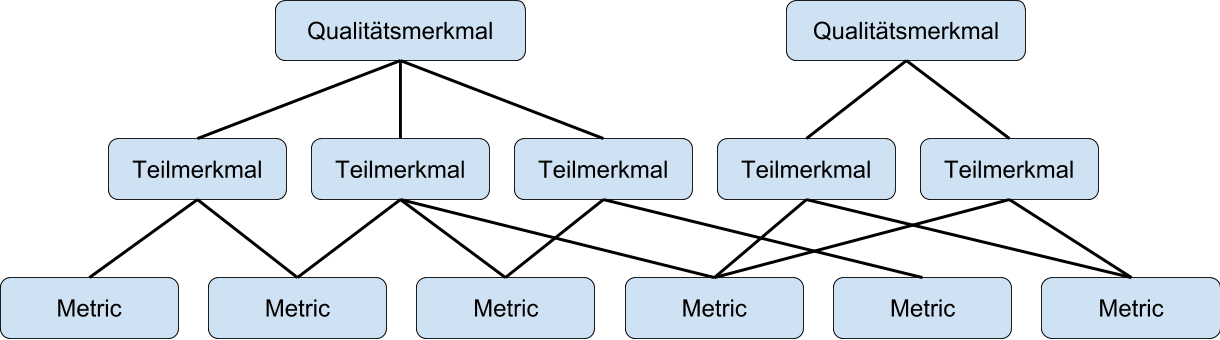
\includegraphics[width=0.9\textwidth]{img/fcm.png}
    \caption{Struktur des \ac{FCM} Modells}\label{fig:fcm}
  \end{figure}
\end{savenotes}

Abbildung~\ref{fig:fcm} zeigt einen solchen Aufbau eines \ac{FCM}-Modells.

\clearpage
\section[\ac{GQM}]{\acf{GQM}~\footcite[][]{basili_goal_nodate}}

\ac{GQM} ist eine Methodik, die dabei hilft, geeignete Metriken für ein Softwareprojekt finden zu können und wurde ursprünglich von der \ac{NASA} entwickelt, um Fehler in bestimmten Projekten zu erkennen.
Der grundlegende Gedanke dahinter ist, dass Metriken ``top\mbox{-}down'' (von oben nach unten) definiert werden müssen.
Dieser Ansatz wird dadurch begründet, dass Metriken sehr viele Charakteristiken abbilden können, aber erst durch Modelle beziehungsweise Ziele richtig genutzt und interpretiert werden können.

Das Ergebnis dieses Modells hat drei Level:
\begin{description}
  \item[GOAL \mbox{-} konzeptuelles Level] \hfill \\ Es werden Ziele für bestimmte Objekte definiert. Objekte können Produkte, Prozesse oder Ressourcen sein.
  \item[QUESTION \mbox{-} operatives Level] \hfill \\ Für jedes Ziel werden Fragen formuliert, die zur Beurteilung oder Erreichung beitragen. Sie versuchen den Grund für die Messung zu charakterisieren.
  \item[METRIC \mbox{-} quantitatives Level] \hfill \\ Jeder Frage werden Metriken zugeordnet, die dabei helfen sollen, sie quantitativ zu beantworten.
\end{description}

\begin{savenotes}
  \begin{figure}[H] 
    \centering
    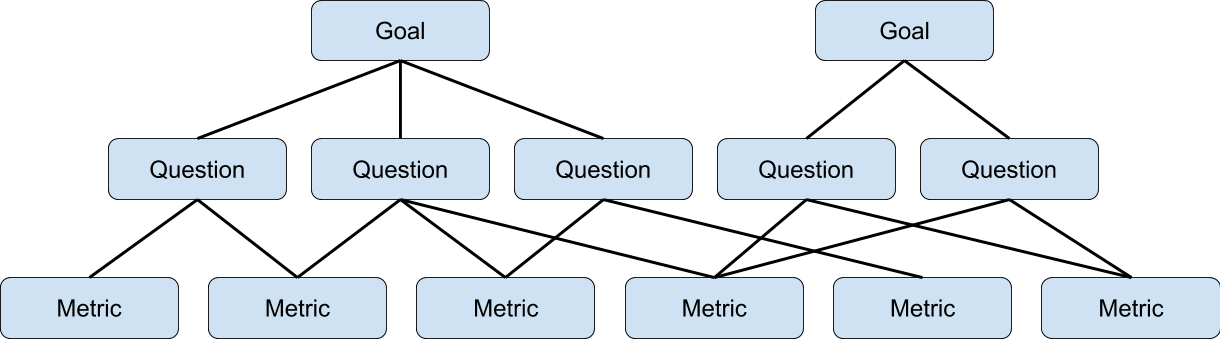
\includegraphics[width=0.9\textwidth]{img/gqm.png}
    \caption{Struktur eines Ergebnisses der \ac{GQM}-Methodik}\label{fig:gqm}
  \end{figure}
\end{savenotes}

Abbildung~\ref{fig:gqm} zeigt die hierarchische Struktur eines Ergebnisses der \ac{GQM}-Methodik.

\subsubsection*{Beispiel~\footcite[][]{basili_goal_nodate}}

Anhand des Beispiels in Tabelle~\ref{tab:gqm-example} soll veranschaulicht werden, wie so ein Ergebnis der \ac{GQM}-Methodik in der Praxis aussehen kann.
Angenommen wird, das Team will seine Zusammenarbeit verbessern. 
Dazu muss das Ziel folgende Punkte spezifizieren: Absicht, Prozess / Produkt / Ressource, Sichtweise und Problem.
Dieses Ziel kann anschließend durch Fragen verfeinert werden.
Aussagen über Zusammenarbeit geben zum Beispiel Pull Requests.
Diese Fragen wiederum können mit Metriken beantwortet werden.
Im Falle der Pull Requests zum Beispiel der Durchschnitt und die Standardabweichung der Kommentare pro Pull Request in jedem Sprint.

\begin{table}[H]
  \centering
  \begin{tabular}{llr}
  GOAL     & \begin{tabular}[c]{@{}l@{}}Absicht\\ Problem\\ Prozess\\ Sichtweise\end{tabular} & \begin{tabular}[c]{@{}l@{}}Verbessern\\ der Zusammenarbeit innerhalb des Teams\\ im Entwicklungsprozess\\ aus Sicht der Entwicklerinnen.\end{tabular} \\ \midrule
  QUESTION & \multicolumn{2}{l}{Wie arbeitet das Team mit Pull Requests?} \\
  METRIC   & \multicolumn{2}{l}{\begin{tabular}[c]{@{}l@{}}Anzahl Pull Requests\\ Anzahl Kommentare pro Pull Request *\\ Anzahl Entwicklerinnen pro Pull Request *\end{tabular}} \\ \midrule
  QUESTION & \multicolumn{2}{l}{Wie viele Entwicklerinnen arbeiten an den einzelnen Modulen?} \\
  METRIC   & \multicolumn{2}{l}{\begin{tabular}[c]{@{}l@{}}Anzahl Commits pro Entwicklerin pro Modul\\ Anzahl Entwicklerinnen pro Pull Request pro Modul *\end{tabular}} \\
  \multicolumn{3}{l}{\begin{tabular}[c]{@{}l@{}} \\ \small{* Durchschnitt und Standardabweichung pro Sprint}\end{tabular}} 
  \end{tabular}
  \caption{Beispiel \ac{GQM}-Methodik}\label{tab:gqm-example}
\end{table}

\chapter{Vorgehensweise}

Agile Methoden, im speziellen Scrum, sind heutzutage in der Softwareentwicklung sehr weit verbreitet.
Ein wichtiges Werkzeug dieser Methoden ist der evolutionäre Ansatz, der in Form von Retrospektiven (bei Scrum) zur kontinuierlichen Verbesserung des agilen Prozesses beitragen soll.
In diesen Retrospektiven werden dann auch Maßnahmen getroffen, um solche Verbesserungen umzusetzen.
In dieser Arbeit soll ein Vorgehensmodell entwickelt werden, wie solche Verbesserungen oder auch Defizite messbar und somit sichtbar gemacht werden können.
Weiters soll eine Software entwickelt werden, um die notwendigen Daten zu sammeln und darstellen zu können.

\section{Vorgehensmodell}

Entwicklung eines Vorgehensmodells zur Bestimmung von relevanten Qualitätsmetriken von agilen Teams.
Dabei müssen folgende Punkte beachtet werden:
\begin{itemize}[noitemsep]
    \item Ebene für die die Metriken bestimmt sind (agiles Team, mittleres Management, Geschäftsleitung)
    \item allgemeine Metriken für diese Ebene
    \item spezielle Probleme erkennen und Metriken dazu erstellen
\end{itemize}

\section{Software}

Entwicklung einer Software zum Sammeln von Kennzahlen zur Erstellung von Qualitätsmetriken. 
Dabei müssen folgende Kriterien beachtet werden:
\begin{itemize}[noitemsep]
    \item Umsetzung in Java
    \item einzubindende Systeme: BitBucket Server~\footcite{bitbucket_server}, JIRA~\footcite{jira}, Jenkins~\footcite{jenkins}, SonarQube~\footcite{sonarqube}, Icinga~\footcite{icinga}
    \item Speicherung und Darstellung der Metriken erfolgt in einem Elastic Stack~\footcite{elastic_stack}
\end{itemize}

\chapter{Umsetzung}

\section{Vorgehensmodell}

\subsection{Metriken Identifizieren}

\subsubsection{\ac{GQM}}

Um eine Vorauswahl an Metriken treffen zu können, wurden alle bisherigen Retrospektiven (es waren genau 15) analysiert und eine Topliste von Schlagwörtern der folgenden Fragestellungen aus den Retrospektiven erstellt:
\begin{enumerate}
    \item Welche guten Entscheidungen haben wir getroffen?
    \item Was haben wir gelernt?
    \item Was können wir besser machen?
    \item Was nervt uns noch immer?
\end{enumerate}

Dazu wurden die Ergebnisse in eine ElasticSearch Datenbank gespeichert und über eine sogenannte Terms Aggregation die wichtigsten Schlagwörter analysiert.
Bei der Indizierung werden die Wörter normalisiert, deshalb die teilweise andere Schreibweise (zum Beispiel wird aus Issue der Term issu).
Die Ergebnisse in Anhang~\ref{appendix:retros} sind für die einzelnen Punkte wie folgt interpretierbar:

\begin{description}
    \item[Welche guten Entscheidungen haben wir getroffen?] \hfill
    \begin{itemize}[noitemsep]
      \item Die ersten fünf Wörter lassen darauf schließen, dass das Team gut zusammenarbeitet, speziell bei der Wissensverteilung: Transparenz, Onboarding von neuen Themen und Pair-Programming.
      \item Ebenfalls lässt sich aus den weiteren Begriffen schließen, dass viel Wert auf Reviews, Daily und die Arbeitsweise an sich gelegt wird.
    \end{itemize}
    \item[Was haben wir gelernt?] \hfill
    \begin{itemize}[noitemsep]
      \item Auch hier spiegelt sich der Daten- und Kommunikationsfluss im Team wider.
      \item Die vielen Scrum Schlagwörter zeigen, dass die Retrospektiven richtig genutzt wurden, um den Prozess zu verbessern.
    \end{itemize}
    \item[Was können wir besser machen?] \hfill
    \begin{itemize}[noitemsep]
      \item Auch hier zeugen die Scrum Schlagwörter wieder von einer Prozessverbesserung und einem selbstreflektiven Verhalten.
      \item Die Dokumentation scheint teilweise noch ein Problem zu sein, diese kommt gleich zweimal vor.
      \item Issues scheinen teilweise nicht optimal zu sein. Da könnte das Schlagwort ``groß'' dazu passen.
      \item ``backlog'', ``blocked'' und ``àblauf'' lassen auf Probleme im Arbeitsablauf schließen.
    \end{itemize}
    \item[Was nervt uns noch immer?] \hfill
    \begin{itemize}[noitemsep]
      \item Hier lassen die Schlagwörter ``updat'', ``erreichbar'', ``infrastruktur'', ``jenkin'', ``test'' und ``umgebung'' auf ein Infrastruktur Problem schließen, welches das Team womöglich ausbremst.
      \item Die Schlagwörter ``lang'', ``groß'' und ``klar'' lassen auf Probleme mit Anforderungen beziehungsweise Stories schließen.
      \item ``apis'', ``dba'', ``laut'' und ``iso'' sind wahrscheinlich äußere Einflüsse, die bei der täglichen Arbeit stören.
    \end{itemize}
  \end{description}

Aus diesen Ergebnissen Lassen sich die \ac{GQM}-Modelle in Tabelle~\ref{tab:gqm-distraction},~\ref{tab:gqm-process} und~\ref{tab:gqm-issues} ableiten.

\begin{table}[H]
    \centering
    \begin{tabular}{llr}
    GOAL     & \begin{tabular}[c]{@{}l@{}}Absicht\\ Problem\\ Ressource\\ Sichtweise\end{tabular} & \begin{tabular}[c]{@{}l@{}}Verringerung\\ der Ablenkung\\ von Entwicklern\\ aus Sicht des Scrum Masters.\end{tabular} \\ \midrule
    QUESTION & \multicolumn{2}{l}{Wie viele Aufgaben erledigt das Team pro Sprint?} \\
    METRIC   & \multicolumn{2}{l}{Aufgaben-Volumen pro Sprint} \\ \midrule
    QUESTION & \multicolumn{2}{l}{Wie viele Aufgaben werden jeden Tag erledigt?} \\
    METRIC   & \multicolumn{2}{l}{\begin{tabular}[c]{@{}l@{}}erledigte Aufgaben pro Tag\\ Burn-down pro Tag\end{tabular}} \\ \midrule
    QUESTION & \multicolumn{2}{l}{Welche Tags haben als ``schlecht'' bewertete Aufgaben?} \\
    METRIC   & \multicolumn{2}{l}{\begin{tabular}[c]{@{}l@{}}Tags der Aufgaben, \\ um ``schlecht'' bewertete besser analysieren zu können\end{tabular}}
    \end{tabular}
    \caption{GQM\mbox{-}Modell \mbox{-} Ablenkung der Entwickler}\label{tab:gqm-distraction}
\end{table}

\begin{table}[H]
    \centering
    \begin{tabular}{llr}
    GOAL     & \begin{tabular}[c]{@{}l@{}}Absicht\\ Problem\\ Prozess\\ Sichtweise\end{tabular} & \begin{tabular}[c]{@{}l@{}}Optimierung\\ des Durchlaufes\\ im Entwicklungsprozess\\ aus Sicht des Scrum Teams.\end{tabular} \\ \midrule
    QUESTION & \multicolumn{2}{l}{Gibt es irgendwelche Engpässe im Prozess?} \\ 
    METRIC   & \multicolumn{2}{l}{Cumulative Flow} \\ \midrule
    QUESTION & \multicolumn{2}{l}{Wie lange dauert der Durchlauf einer Aufgabe?} \\
    METRIC   & \multicolumn{2}{l}{Lead Time}
    \end{tabular}
    \caption{GQM\mbox{-}Modell \mbox{-} Schwachstellen im Prozess}\label{tab:gqm-process}
\end{table}

\begin{table}[H]
    \centering
    \begin{tabular}{llr}
    GOAL     & \begin{tabular}[c]{@{}l@{}}Absicht\\ Problem\\ Ressource\\ Sichtweise\end{tabular} & \begin{tabular}[c]{@{}l@{}}Optimierung\\ der Aufgabengröße\\ im Backlog\\ aus Sicht des Product Owners.\end{tabular} \\ \midrule
    QUESTION & \multicolumn{2}{l}{Wie groß ist die Aufgabengröße im Durchschnitt?} \\
    METRIC   & \multicolumn{2}{l}{erledigte Story-Points / Aufgaben-Volumen} \\ \midrule
    QUESTION & \multicolumn{2}{l}{Wie lange dauert der Durchlauf einer Aufgabe?} \\
    METRIC   & \multicolumn{2}{l}{Lead-Time} \\ \midrule
    QUESTION & \multicolumn{2}{l}{Wie viele Aufgaben gehen im Entwicklungsprozess rückwärts?} \\
    METRIC   & \multicolumn{2}{l}{Aufgaben-Rückfälligkeit}
    \end{tabular}
    \caption{GQM\mbox{-}Modell \mbox{-} Aufgabengröße}\label{tab:gqm-issues}
\end{table}

\subsubsection{Umfrage im Team}

Zusätzlich zu der Analyse der Retrospektiven wurden dem Team Metriken und die Fragen, die damit beantwortet werden können, in Form einer Umfrage vorgestellt.
Die einzelnen Metriken wurden von den Teammitgliedern nach Wichtigkeit mit einer Skala von 1 bis 10 bewertet.
Anhang~\ref{appendix:questions} zeigt die Umfrage, wie sie den Teammitgliedern vorgelegt wurde und Anhang~\ref{appendix:answers} die dazugehörigen Antworten.
Die Ergebnisse wurden nach ihrem Druchschnittwert sortiert und die 10 als am wichtigsten bewerteten Metriken sind:

\begin{itemize}[noitemsep]
    \item \textbf{Burn Down (9,00)} \mbox{-} Erfüllt das Team seine Commitments? Plant das Team seine Arbeit realistisch?
    \item \textbf{Velocity (9,00)} \mbox{-} Wie konsistent arbeitet das Team?
    \item \textbf{Aufgaben-Volumen (8,57)} \mbox{-} Wie viel ungeplante Arbeit kam zum Sprint dazu? Wie groß ist die durchschnittliche Aufgabe? Gibt es Ausreißer?
    \item \textbf{Cumulative Flow (8,29)} \mbox{-} Gibt es Engpässe oder Schwachstellen im Prozess? Müssen gewisse Abläufe im Prozess optimiert werden?
    \item \textbf{Lead Time (8,14)} \mbox{-} Wie schnell können Aufgaben vom Team erledigt werden? Wie lange dauert die Umsetzung eines neuen Features?
    \item \textbf{Stresstests oder Benchmarking (7,86)} \mbox{-} Ist das Produkt auch noch unter Last verwendbar? Wie verändert sich die Leistung über die Zeit?
    \item \textbf{Code Coverage (7,71)} \mbox{-} Gibt es Module, die nicht oder schlecht getestet sind? Wie sieht die Entwicklung der Testabdeckung über die Zeit aus?
    \item \textbf{Bug Counts (7,57)} \mbox{-} Wie viele Fehler werden vom Team im Entwicklungsprozess übersehen? Wie viel ungeplante Arbeit kam zum Sprint dazu?
    \item \textbf{Aufgaben-Rückfälligkeit (7,57)} \mbox{-} Wie viele Aufgaben werden wieder in einen vorhergehenden Status gesetzt? Gibt es Probleme beim Verständnis der Aufgaben? Wie klar sind die Erwartungen des Teams an eine abgeschlossene Änderung (DoD)?
    \item \textbf{Bug-Erzeugungsrate (7,43)} \mbox{-} Wie viele Fehler wurden zu einem bestimmten Zeitpunkt erzeugt?
\end{itemize}

Zusätzlich wurde in den offenen Fragen am Ende zwiemal gefordert, dass die Flüchtigkeit von Anforderungen Sichtbar wird. 
Dies kann zum einen durch die oben genannte Aufgaben-Rückfälligkeit und andererseits durch folgende Metrik abgebildet werden:

\begin{itemize}[noitemsep]
    \item \textbf{Anforderungen-Flüchtigkeit} \mbox{-} Wie oft wurde die Anforderung der Aufgabe angepasst?
\end{itemize}

\section{Software}

Technologien, Plattform, etc.

\subsection{Architektur}

Abbildung~\ref{fig:position_architecture} zeigt die Position und Abbildung~\ref{fig:overview_architecture} die grobe Architektur der Software (Agile Metrics).
Die Software bildet eine Schnittstelle zwischen den einzelnen Systemen des Entwicklungsprozesses und dem System zur Darstellung der Metriken (in diesem Fall ElasticSearch und Kibana).

\begin{savenotes}
    \begin{figure}[H] 
        \centering
            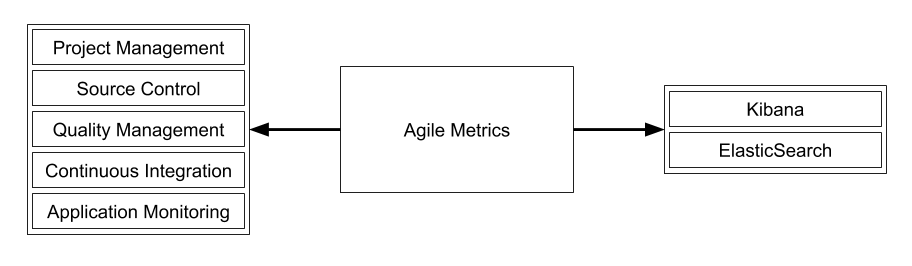
\includegraphics[width=0.8\textwidth]{img/position-overview.png}
        \caption{Position der Software}\label{fig:position_architecture}
    \end{figure}
\end{savenotes}

\begin{savenotes}
    \begin{figure}[H] 
        \centering
            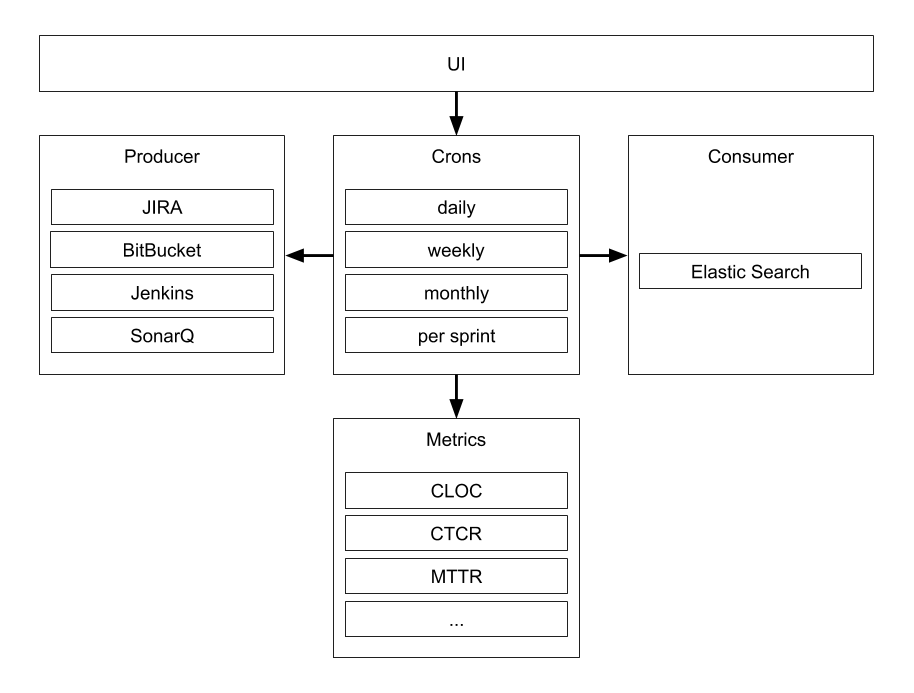
\includegraphics[width=0.8\textwidth]{img/architecture-overview.png}
        \caption{Übersicht der Software-Architektur}\label{fig:overview_architecture}
    \end{figure}
\end{savenotes}

\begin{description}
    \item[UI] \hfill \\ Bietet eine grafische Benutzeroberfläche zur Konfiguration.
    \item[Producer] \hfill \\ Sind Schnittstellen zu allen Systemen, die Messdaten erzeugen.
    \item[Crons] \hfill \\ Zeitsteuerung der Messdaten-Abfrage (z.B. täglich oder pro Sprint).
    \item[Metrics] \hfill \\ Hier können aus Messdaten direkt Metriken erstellt werden.
    \item[Consumer] \hfill \\ Sind Schnittstellen zu allen Systemen, die Messdaten und Metriken konsumieren.
\end{description}

\chapter{Ergebnisse}

\section{Vorgehensmodell}

\ldots Ergebnis der Ausarbeitung.

\section{Einführung des Vorgehensmodells}

\ldots bei Gebrüder Weiss.

\section{Inbetriebnahme der Software}

\ldots allgemein, Beschreibung der Connectoren, Darstellungsarten, etc.

\subsection{Visualisierte Ergebnisse}

\begin{savenotes}
    \begin{figure}[H] 
        \centering
            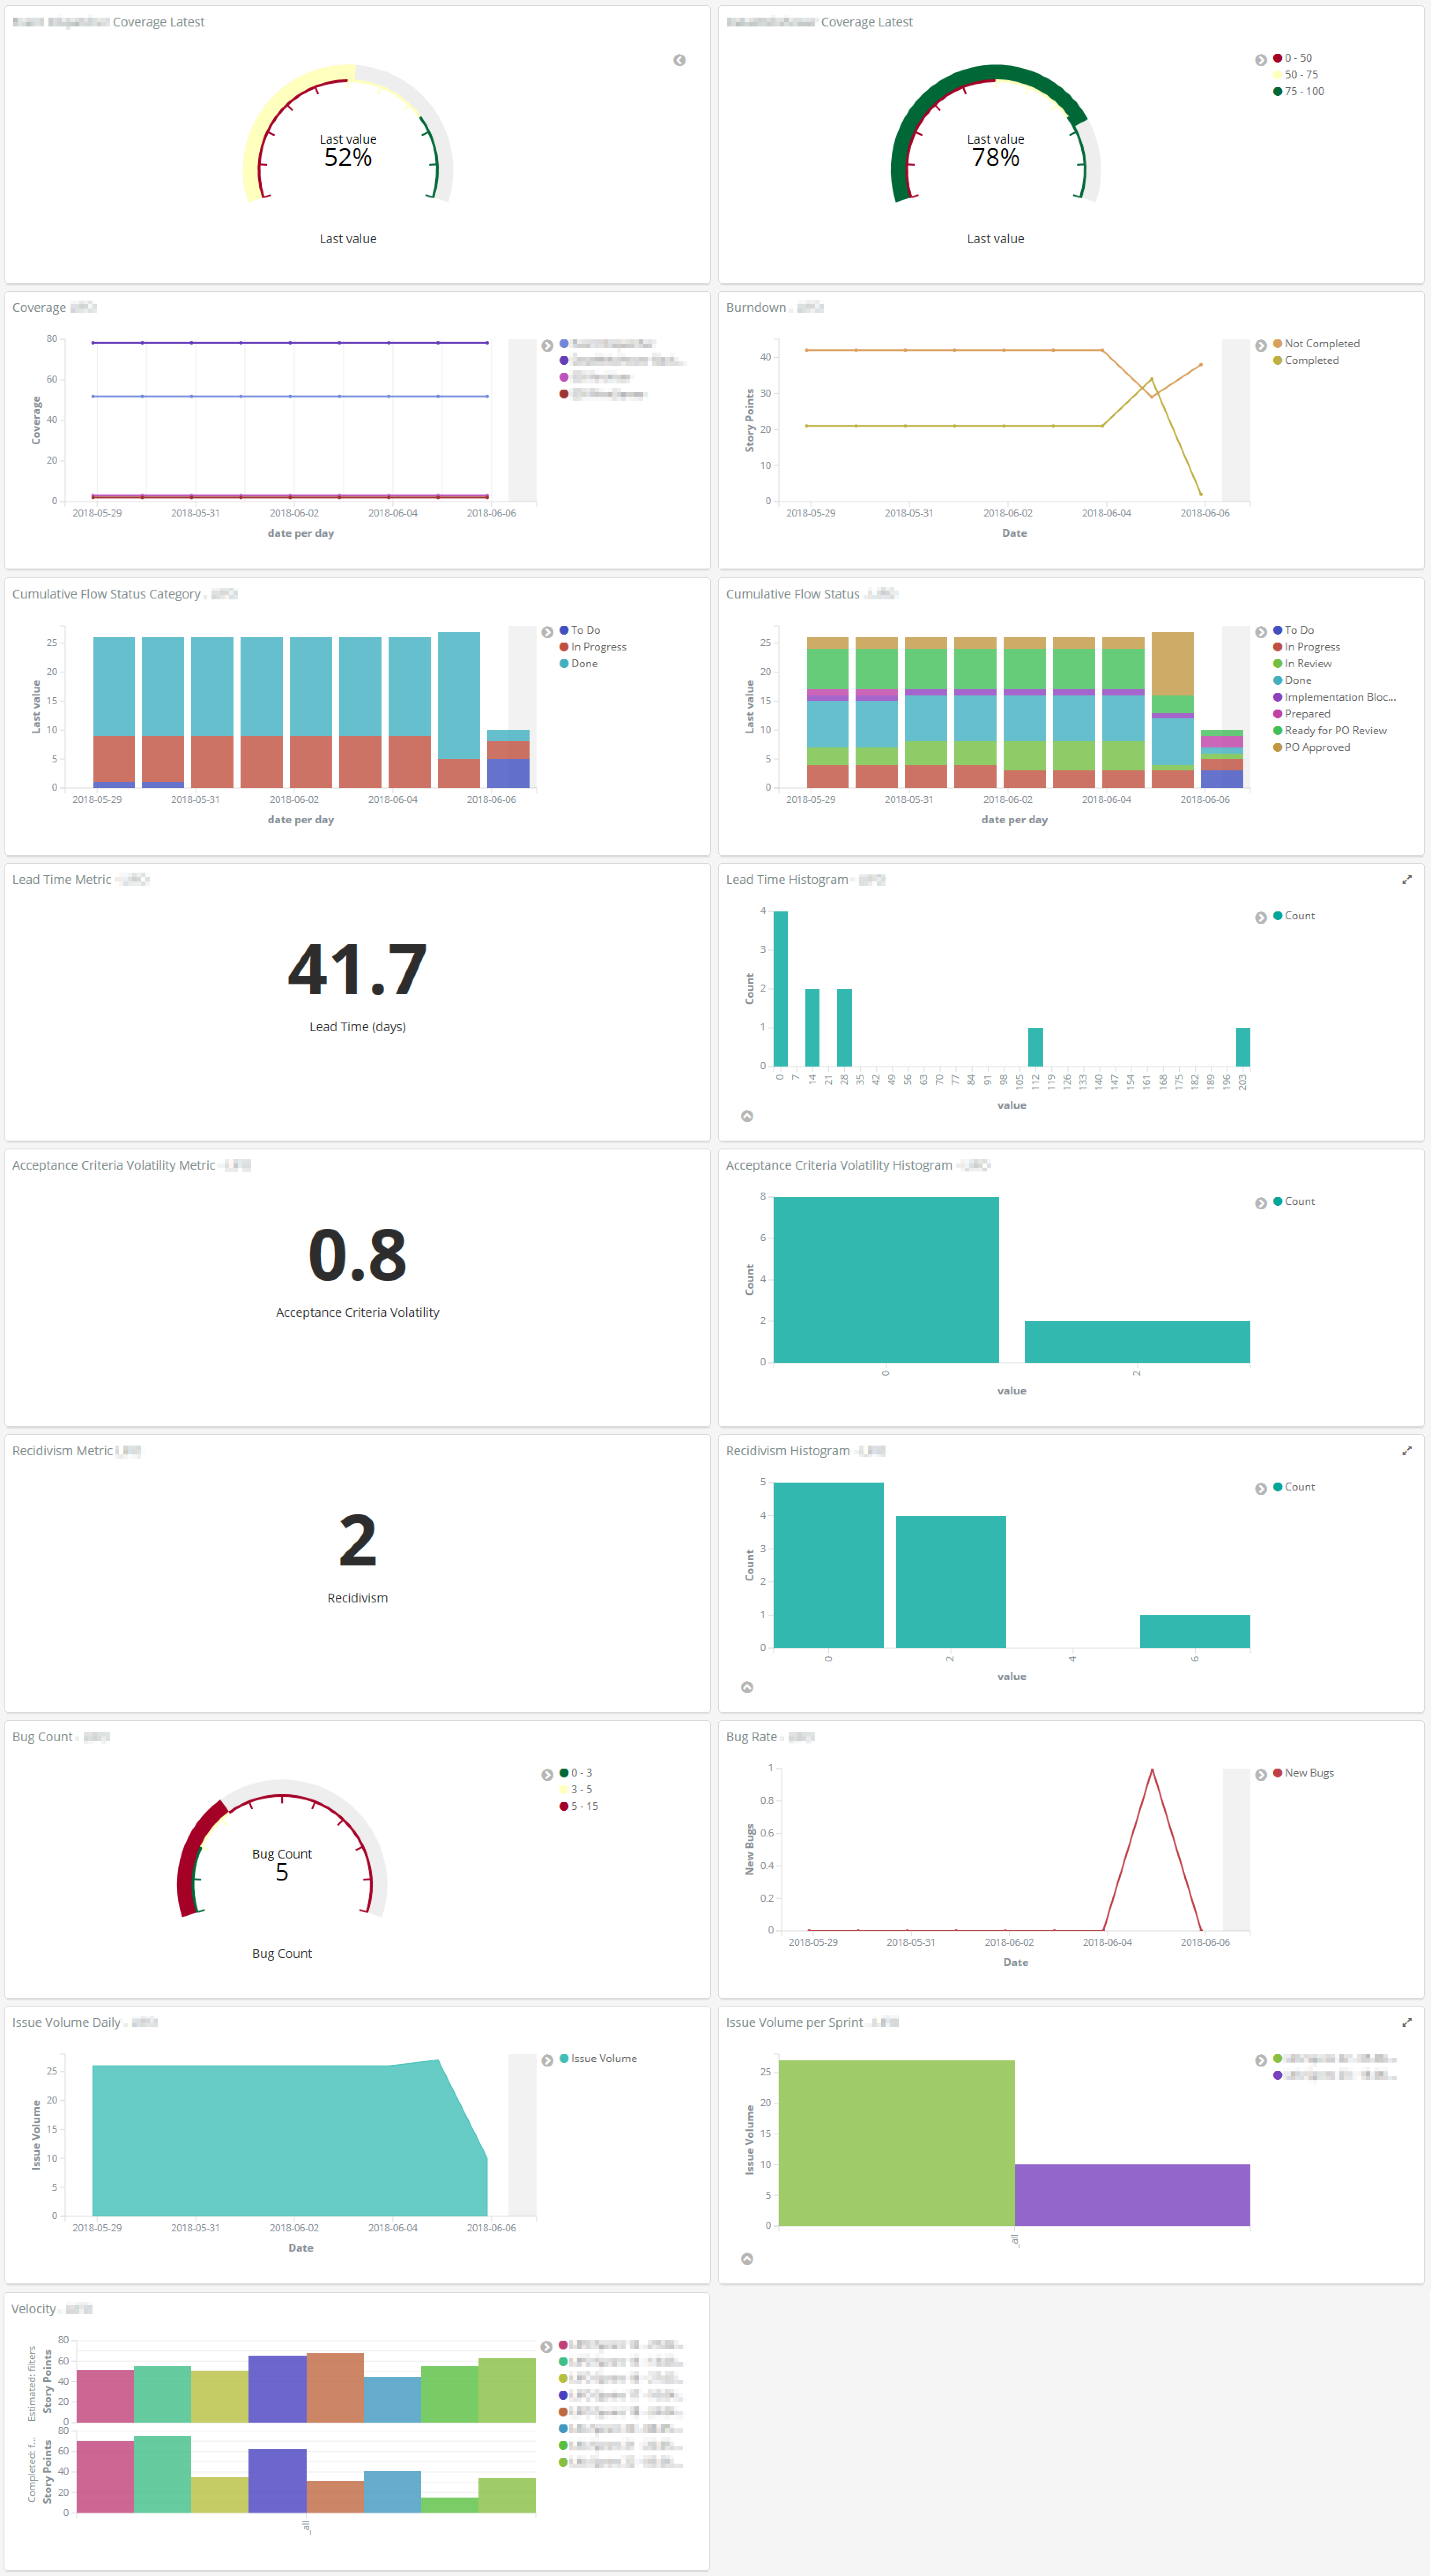
\includegraphics[width=1.0\textwidth]{img/dashboard.png}
        \caption{Dashboard mit den Metriken}\label{fig:dashboard}
    \end{figure}
\end{savenotes}

\section{Evaluierung des Vorgehensmodells}

\ldots wie wurde es angenommen? Welche Auswirkungen hatte es?

\chapter{Schlussfolgerungen}

In dieser Arbeit konnte gezeigt werden, dass mithilfe des \ac{GQM}-Modells, ergänzt durch eine Umfrage im entsprechenden Scrum Team, Metriken ermittelt werden können, die es ermöglichen, die Schwachstellen in einem Produkt und im agilen Prozess in Zahlen zu fassen.
Diese Metriken ermöglichen es dem agilen Team, seine Fortschritte bei den Retrospektiven nachvollziehbar bewerten und weitere Maßnahmen treffen zu können.
Außerdem können durch die Kombination unterschiedlicher Metriken Korrelationen zwischen bestimmten Metriken nachgewiesen oder widerlegt werden.
Reichen die bekannten Metriken in der Literatur nicht aus, können auch eigene erstellt werden.
\\
Die entwickelte Software hilft dabei, die Daten aus den unterschiedlichen Systemen im Entwicklungsprozess als Metriken aufzubereiten und zu speichern.
Dabei wurde bei der Architektur auf Fehlertoleranz und einfache Erweiterbarkeit geachtet, sodass ein einfacher Betrieb und eine Erweiterung der unterstützten Systeme und Metriken möglich ist.
Für einen einfachen Zugang und eine uneingeschränkte Erweiterbarkeit wurde der Quellcode der Software unter der quelloffenen MIT-Lizenz veröffentlicht.
Bei der Visualisierung von Metriken bietet Kibana eine geeignete Plattform, um aus den gespeicherten Metriken einfach Dashboards mit unterschiedlichen Visualisierungen bereitzustellen.
Dabei muss berücksichtigt werden, dass Entwicklerinnen, Scrum Master und Product Owner jeweils unterschiedliche Interessen an den Metriken haben.
Durch eine geeignete Gruppierung der Metriken können den unterschiedlichen Teammitgliedern auf einen Blick die wichtigsten Metriken dargestellt werden.
Dadurch wird das Dashboard auch regelmäßig genutzt und somit die Akzeptanz noch weiter erhöht.
Der Einsatz der Software ermöglicht den Aufbau einer zentralen Stelle, an der die Metriken aus allen relevanten System gesammelt, dargestellt und kombiniert werden können.
\\
Schwachstellen wurden bei der Art der Darstellung mancher Metriken identifiziert.
Hier war der Wunsch nach einer besseren Beschreibung der Metriken, um Diskussionen über deren Bedeutung zu vermeiden.
Zusätzlich soll eine Beschreibung von Zielen helfen, die Absicht hinter Metriken beschreiben zu können.
Bei manchen Darstellungen wurden noch zusätzliche Detailinformationen zu den einzelnen Datensätzen gewünscht, um Ausreißer leichter identifizieren zu können.
Trotzdem wurde das erstellte Dashboard trotz des relativ kurzen Testzeitraums von nicht ganz drei Sprints gut angenommen.
Bei der Evaluierung wurde auch klar, dass die Teammitglieder bereits erkannten, wie sie das Dashboard persönlich am besten nutzen.
\\
Durch den Einsatz der entwickelten Software und der vorgestellten Modelle zur Identifizierung von relevanten Metriken, kann die Qualität in einem agilen Team dadurch erhöht werden, dass Qualitätsprobleme durch Metriken sichtbar gemacht und in den Retrospektiven Gegenmaßnahmen dafür getroffen werden können.

\chapter{Zusammenfassung}

Scrum ist inzwischen eine sehr weit verbreitete agile Vorgehensweise von Entwicklungsteams.
Dabei ist die Reflexion der bisherigen Arbeit eine der Grundideen von Scrum, der sogenannte Empirismus.
Empirismus ist die Theorie, dass Wissen aus Erfahrung erlangt wird.
Um auf Basis dieses Wissens Entscheidungen zu treffen, benötigt ein Scrum-Team Kennzahlen.
Solche Kennzahlen können in Form von Metriken in einem leicht zugänglichen Dashboard visualisiert werden.
Metriken dienen hauptsächlich dazu, Qualitätsmerkmale eines Produkts oder Prozesses als Zahlenwert darzustellen.
\\
Eingeführt wurde ein solches Dashboard bei einem relativ fortgeschrittenen Scrum-Team in einem Unternehmen mit rund 6700 Mitarbeitern.
Gestartet wurde mit der Ermittlung von geeigneten Metriken für das Team.
Dazu wurden zuerst alle bisherigen Retrospektiven ausgewertet und basierend auf diesen Daten mit der \ac{GQM}-Methodik Metriken ermittelt.
Zusätzlich wurde aufgrund des erfahrenen Teams noch eine Umfrage gemacht, bei der den Teammitgliedern die gängigsten Metriken vorgestellt und in einer Skala von eins bis zehn nach Wichtigkeit bewertet wurden.
\\
Um diese ermittelten Metriken dann darzustellen, wurde eine leicht erweiterbare, quelloffene Software in Java erstellt, die alle relevanten Daten aus den Systemen im Entwicklungsprozess über Schnittstellen sammelt, aufbereitet und als Metriken in einer Datenbank speichert.
Konkret wurde der sogenannte Elastic Stack eingesetzt, also eine ElasticSearch Datenbank zur Speicherung und Kibana zur Visualisierung der Metriken und Bereitstellung über Dashboards.
Diese Metriken wurden anschließend vom Scrum-Team über den Zeitraum von nicht ganz drei Sprints getestet.
Dabei konnte gezeigt werden, dass je nach Rolle im Team zwar andere Metriken wichtig sind, aber jeder das Dashboard für sich zu nutzen wusste.
Besonders der Scrum-Master bekam schnell einen Eindruck, welche Möglichkeiten dem Team dadurch eröffnet werden.

\section*{Ausblick}

Folgende Erweiterungen dieser Arbeit wären möglich:

\begin{description}
    \item[Testzeitraum] \hfill \\ Die Entwicklung des Teams und des Dashboards mit den Metriken könnte noch über einen längeren Zeitraum verfolgt werden, um ausführlichere Rückschlüsse über die Effektivität und den Nutzen zu ziehen.
    \item[Testumfang] \hfill \\ Der Testumfang kann auf mehrere Teams erweitert werden, um ein noch umfangreicheres Feedback zu bekommen.
    \item[Systeme] \hfill \\ Mehr unterstützte Systeme kann die Akzeptanz der Software erhöhen.
    \item[Metriken] \hfill \\ Auch neue Metriken erhöhen die Akzeptanz der Software und erlauben es Teams, noch mehr Einsicht in ihre Prozesse und Systeme zu erlangen.
    \item[Geschäftsebenen] \hfill \\ Das Dashboard könnte noch weiteren Ebenen im Unternehmen bereitgestellt werden, zum Beispiel dem Management, um eine Übersicht über den Gesamtprozess zu erlangen.
\end{description}


% Literaturverzeichnis:
\clearpage
\phantomsection{}
\addcontentsline{toc}{chapter}{Literaturverzeichnis}
\printbibliography{}

\appendix
\addchap{Anhang}
\refstepcounter{chapter}

\section{Metriken aus dem Entwicklungsprozess}\label{appendix:metrics}

\begin{table}[H]
    \centering
    \begin{tabular}{p{6.5cm}p{8cm}} \toprule
    \textbf{\ac{CLOC}} & Anzahl der geänderten Zeilen im Quellcode. \\
    \multicolumn{2}{p{14.5cm}}{\textit{Wie viele Änderungen passieren in der Codebasis? \newline Wo finden die meisten Änderungen statt?}} \\ \midrule
    \textbf{\ac{CLOC} pro Entwickler} & Anzahl der geänderten Zeilen im Quellcode pro Entwickler. \\ 
    \multicolumn{2}{p{14.5cm}}{\textit{Wie viel Code ändert jeder im Team? \newline  Wer ist wie oft in welchem Modul?}} \\ \midrule
    \textbf{\ac{CLOC} pro Commit} & Anzahl der geänderten Zeilen im Quellcode pro Commit. \\ 
    \multicolumn{2}{p{14.5cm}}{\textit{Wie groß sind die Commits?}} \\ \midrule
    \textbf{Commits} & Gesamtzahl an Commits in einem bestimmten Zeitraum. \\ 
    \multicolumn{2}{p{14.5cm}}{\textit{Wie viel Änderungen wurden im Quellcode vorgenommen?}} \\ \midrule
    \textbf{Commits pro Entwickler} & Gesamtzahl an Commits in einem bestimmten Zeitraum pro Entwickler. \\ 
    \multicolumn{2}{p{14.5cm}}{\textit{Wie viel Änderungen wurden im Quellcode von einem Entwickler vorgenommen?}} \\ \midrule
    \textbf{Kommentare pro Commit} & Anzahl der Kommentare pro Commit. \\ 
    \multicolumn{2}{p{14.5cm}}{\textit{Wer arbeitet zusammen? \newline Wie viel wird zusammengearbeitet?}} \\ \midrule
    \textbf{Pull Requests} & Gesamtzahl an Pull Requests in einem bestimmten Zeitraum. \\ 
    \multicolumn{2}{p{14.5cm}}{\textit{Wird mit Pull Requests gearbeitet? \newline Werden Reviews gemacht?}} \\ \midrule
    \textbf{Gemergte Pull Requests} & Anzahl erfolgreicher Pull Requests in einem bestimmten Zeitraum. \\ 
    \multicolumn{2}{p{14.5cm}}{\textit{Wie oft werden erfolgreiche Änderungen in die Codebasis übernommen?}} \\ \midrule
    \textbf{Abgelehnte Pull Requests} & Anzahl abgelehnter Pull Requests in einem bestimmten Zeitraum. \\ 
    \multicolumn{2}{p{14.5cm}}{\textit{Wie oft werden Änderungen an der Codebasis abgelehnt? \newline Wie klar sind die Erwartungen des Teams an eine abgeschlossene Änderung (\ac{DoD})?}} \\ \midrule
    \textbf{Kommentare pro Pull Request} & Anzahl der Kommentare pro Pull Request. \\ 
    \multicolumn{2}{p{14.5cm}}{\textit{Wer arbeitet zusammen? \newline Wie viel wird zusammengearbeitet?}} \\ \bottomrule
    \end{tabular}
    \caption{Kennzahlen aus dem \ac{VCS}}\label{metrics-table-vcs}
  \end{table}
  
  \begin{table}[H]
    \centering
    \begin{tabular}{p{5cm}p{9.5cm}} \toprule
    \textbf{Burn Down} & Die Anzahl erledigte Arbeit über die Zeit. Liefert einen Richtwert, wo man sich gerade im Sprint befindet, verglichen zum Commitment. \\
    \multicolumn{2}{p{14.5cm}}{\textit{Erfüllt das Team seine Commitments? \newline Plant das Team seine Arbeit realistisch?}} \\ \midrule
    \textbf{Velocity} & Eine relative Messung der Konsistenz erledigter Arbeit über die Sprints. \\
    \multicolumn{2}{p{14.5cm}}{\textit{Wie konsistent arbeitet das Team?}} \\ \midrule
    \textbf{Cumulative Flow} & Zeigt wie viel Aufgaben nach Status dem Team zugewiesen sind über die Zeit. \\
    \multicolumn{2}{p{14.5cm}}{\textit{Gibt es Engpässe oder Schwachstellen im Prozess? \newline Müssen gewisse Abläufe im Prozess optimiert werden?}} \\ \midrule
    \textbf{Lead Time} & Zeit zwischen Start und Abschluss einer Aufgabe, vor allem interessant bei Kanban. \\
    \multicolumn{2}{p{14.5cm}}{\textit{Wie schnell können Aufgaben vom Team erledigt werden? \newline Wie lange dauert die Umsetzung eines neuen Features?}} \\ \midrule
    \textbf{Bug Counts} & Die Anzahl an Bugs über die Zeit. \\
    \multicolumn{2}{p{14.5cm}}{\textit{Wie viele Fehler werden vom Team im Entwicklungsprozess übersehen? \newline Wie viel ungeplante Arbeit kam zum Sprint dazu?}} \\ \midrule
    \textbf{Bug-Erzeugungsrate} & Anzahl Bugs nach Erstellungsdatum. \\
    \multicolumn{2}{p{14.5cm}}{\textit{Wie viele Fehler wurden zu einem bestimmten Zeitpunkt erzeugt?}} \\ \midrule
    \textbf{Bug-Fertigstellungsrate} & Anzahl Bugs nach Erledigungsdatum. \\
    \multicolumn{2}{p{14.5cm}}{\textit{Wie viele Fehler wurden zu einem bestimmten Zeitpunkt beseitigt?}} \\ \midrule
    \textbf{Aufgaben-Volumen} & Ist die Anzahl der Aufgaben und kann der Schätzung gegenübergestellt werden, um die Größe der Aufgaben oder ungeplante Arbeit aufzuzeigen. \\
    \multicolumn{2}{p{14.5cm}}{\textit{Wie viel ungeplante Arbeit kam zum Sprint dazu? \newline Wie groß ist die durchschnittliche Aufgabe? Gibt es Ausreißer?}} \\ \midrule
    \textbf{Aufgaben-Rückfälligkeit} & Zeigt auf, wie oft Aufgaben im Arbeitsablauf rückwärts gehen. \\
    \multicolumn{2}{p{14.5cm}}{\textit{Wie viele Aufgaben werden wieder in einen vorhergehenden Status gesetzt? \newline Gibt es Probleme beim Verständnis der Aufgaben? \newline Wie klar sind die Erwartungen des Teams an eine abgeschlossene Änderung (DoD)?}} \\ \bottomrule
    \end{tabular}
    \caption{Kennzahlen aus dem \ac{PTS}}\label{metrics-table-pts}
  \end{table}
  
  \begin{table}[H]
    \centering
    \begin{tabular}{p{6.5cm}p{8cm}} \toprule
    \textbf{Build-Dauer} & Geschätzte und tatsächliche Dauer der Builds. \\
    \multicolumn{2}{p{14.5cm}}{\textit{Wie lange dauert es ein Software-Artefakt zu erstellen? \newline Wie verändert sich die Dauer der Erstellung eines Software-Artefakts über die Zeit?}} \\ \midrule
    \textbf{Build-Status} & Es können die Anzahl der erfolgreichen und fehlerhaften Builds gegenüber gestellt werden. \\
    \multicolumn{2}{p{14.5cm}}{\textit{Gibt es ein Problem im Freigabeprozess?}} \\ \midrule
    \textbf{Build-Frequenz} & Wie oft wird ein Build ausgelöst. \\
    \multicolumn{2}{p{14.5cm}}{\textit{Wird oft genug ein neues Software-Artefakt erstellt?}} \\ \midrule
    \textbf{Test Reports} & Anzahl erfolgreicher und fehlerhafter Tests, Gesamtdauer der Tests. \\
    \multicolumn{2}{p{14.5cm}}{\textit{Wie lange dauert ein kompletter Testdurchlauf? \newline Gibt es Tests, die optimiert werden müssen? \newline Wie oft werden fehlerhafte Tests in die Codebasis aufgenommen?}} \\ \midrule
    \textbf{Code Coverage} & Wie viel Prozent des Quellcodes ist mit Tests abgedeckt. \\
    \multicolumn{2}{p{14.5cm}}{\textit{Gibt es Module, die nicht oder schlecht getestet sind? \newline Wie sieht die Entwicklung der Testabdeckung über die Zeit aus?}} \\ \midrule
    \textbf{Stresstests oder Benchmarking} & Hier kann das Ergebnisse die unterschiedliche Reports sein. \\
    \multicolumn{2}{p{14.5cm}}{\textit{Ist das Produkt auch noch unter Last verwendbar? \newline Wie verändert sich die Leistung über die Zeit?}} \\ \bottomrule
    \end{tabular}
    \caption{Kennzahlen aus den \ac{CI}- und \ac{CD}}-Systemen\label{metrics-table-cicd}
  \end{table}
  
  \begin{table}[H]
    \centering
    \begin{tabular}{p{5cm}p{9.5cm}} \toprule
    \textbf{CPU Nutzung} & Auslastung der Prozessoren über die Zeit. \\
    \textbf{Heap Size} & Auslastung des Heap über die Zeit. \\
    \multicolumn{2}{p{14.5cm}}{\textit{Arbeitet die Software technisch effizient? \newline Ist die Hardware ausreichend? \newline Gibt es eine erhöhte Auslastung nach einer Änderung?}} \\ \midrule
    \textbf{Fehlerraten} & Anzahl Fehler über die Zeit (kann aus dem Logging kommen). \\
    \multicolumn{2}{p{14.5cm}}{\textit{Werden seit einer Änderung mehr Fehler produziert? \newline Wie entwickelt sich die Fehlerrate über die Zeit?}} \\ \midrule
    \textbf{Antwortzeiten} & Dauer der Verarbeitung bestimmter Anfragen. \\
    \multicolumn{2}{p{14.5cm}}{\textit{Reagiert und arbeitet das Produkt noch schnell genug? \newline Gibt es Geschwindigkeitsprobleme seit der letzten Änderung? \newline Wie entwickeln sich die Antwortzeiten über die Zeit?}} \\ \midrule
    \textbf{Benutzeranzahl} & Anzahl gleichzeitiger Benutzer in der Applikation über die Zeit. \\
    \multicolumn{2}{p{14.5cm}}{\textit{Wie entwickeln sich die Nutzerzahlen mit der Zeit? \newline Geht das Produkt in die richtige Richtung? \newline Ist mit höheren Lasten zu rechnen?}} \\ \midrule
    \textbf{Aufenthaltsdauer} & Verweildauer der Benutzer auf bestimmten Seiten. \\
    \multicolumn{2}{p{14.5cm}}{\textit{Welche Features werden besonders oft / selten genutzt? \newline Hat das neue Feature den gewünschten Effekt? Wird es genutzt?}} \\ \midrule
    \textbf{Conversion Rate} & Anzahl Benutzer die zu Kunden wurden. \\
    \multicolumn{2}{p{14.5cm}}{\textit{Wie entwickelt sich die Zahl der zahlenden Neukunden?}} \\ \midrule
    \textbf{Semantisches Logging} & Strukturierte Daten aus dem Logging. \\
    \multicolumn{2}{p{14.5cm}}{\textit{Hier können Daten zu anderen Fragen gesammelt werden, die für den Prozess wichtig sind.}} \\ \bottomrule
    \textbf{Verfügbarkeit} & Verfügbarkeit der Applikation über die Zeit. \\
    \multicolumn{2}{p{14.5cm}}{\textit{Wie hoch ist die Ausfallsicherheit? \newline Wie lange war die Applikation nicht verfügbar?}} \\ \bottomrule
    \end{tabular}
    \caption{Kennzahlen aus den \ac{APM}- und \ac{BI}}-Systemen\label{metrics-table-apm}
  \end{table}

\newpage
\section{Ergebnisse Analyse Retrospektiven}\label{appendix:retros}

\subsection*{Welche guten Entscheidungen haben wir getroffen?}
\begin{enumerate}
    \item sprint (4)
    \item einblick (3)
    \item onboarding (3)
    \item pair (3)
    \item programming (3)
    \item system (3)
    \item arbeit (2)
    \item daily (2)
    \item erledig (2)
    \item information (2)
    \item issu (2)
    \item po (2)
    \item review (2)
    \item reviewing (2)
    \item schnell (2)
    \item stori (2)
    \item urlaub (2)
    \item angenehm (1)
    \item annehm (1)
    \item cloud (1)
    \item dailys (1)
    \item diskussion (1)
    \item dor (1)
    \item durchgefuhrt (1)
    \item einfach (1)
\end{enumerate}

\subsection*{Was haben wir gelernt?}
\begin{enumerate}
    \item sprint (7)
    \item onboarding (4)
    \item team (4)
    \item arbeit (3)
    \item besprech (3)
    \item board (3)
    \item datenfluss (3)
    \item issus (3)
    \item planungswoch (3)
    \item retro (3)
    \item richtlini (3)
    \item system (3)
    \item uberblick (3)
    \item umgestellt (3)
    \item altlast (2)
    \item analogboard (2)
    \item approved (2)
    \item backlog (2)
    \item daily (2)
    \item digital (2)
    \item direkt (2)
    \item genau (2)
    \item impediment (2)
    \item infrastruktur (2)
    \item iso (2)
\end{enumerate}

\subsection*{Was können wir besser machen?}
\begin{enumerate}
    \item sprint (10)
    \item review (7)
    \item checklist (4)
    \item daily (4)
    \item display (4)
    \item doku (4)
    \item issu (4)
    \item po (4)
    \item einarbeitung (3)
    \item einkalkuli (3)
    \item gross (3)
    \item https (3)
    \item java (3)
    \item stori (3)
    \item ablauf (2)
    \item anderung (2)
    \item arbeitspaket (2)
    \item aufnehm (2)
    \item aufteil (2)
    \item backlog (2)
    \item blocked (2)
    \item dokumenti (2)
    \item erledig (2)
    \item geplant (2)
    \item geschatzt (2)
\end{enumerate}

\subsection*{Was nervt uns noch immer?}
\begin{enumerate}
    \item problem (11)
    \item updat (11)
    \item apis (10)
    \item archiv (10)
    \item erreichbar (10)
    \item infrastruktur (10)
    \item jenkin (10)
    \item test (9)
    \item umgebung (9)
    \item dba (8)
    \item eingerichtet (8)
    \item jndi (8)
    \item laut (8)
    \item verwendbar (8)
    \item arbeit (7)
    \item impediment (7)
    \item iso (7)
    \item lang (7)
    \item mitarbeit (6)
    \item mehr (5)
    \item wichtig (5)
    \item anderung (4)
    \item aufteilbar (4)
    \item gross (4)
    \item klar (4)
\end{enumerate}

\newpage
\section{Umfrage Scrum Team}

\subsection{Fragebogen}\label{appendix:questions}
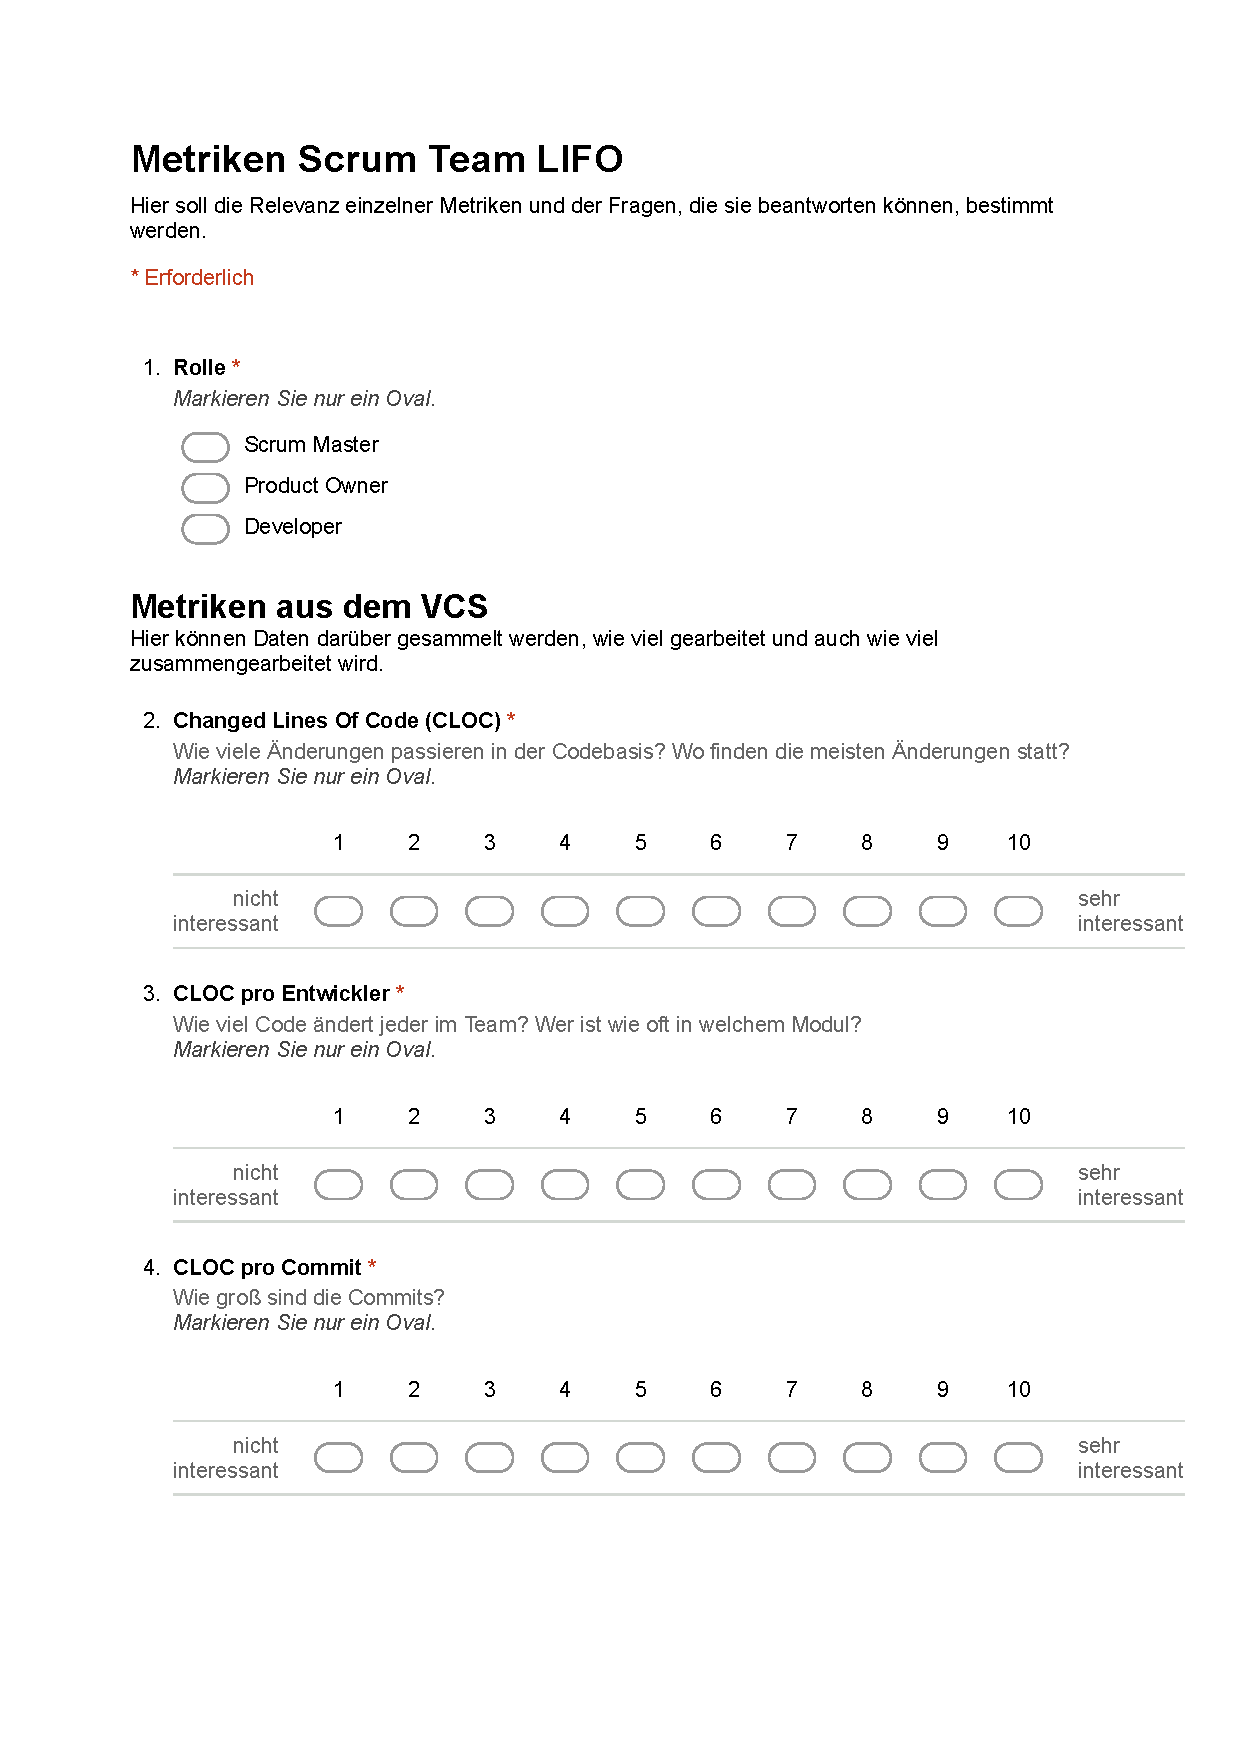
\includepdf[pages=-, scale=0.9, pagecommand={\thispagestyle{plain}}]{appendix/fragebogen.pdf}

\subsection{Ergebnisse}\label{appendix:answers}
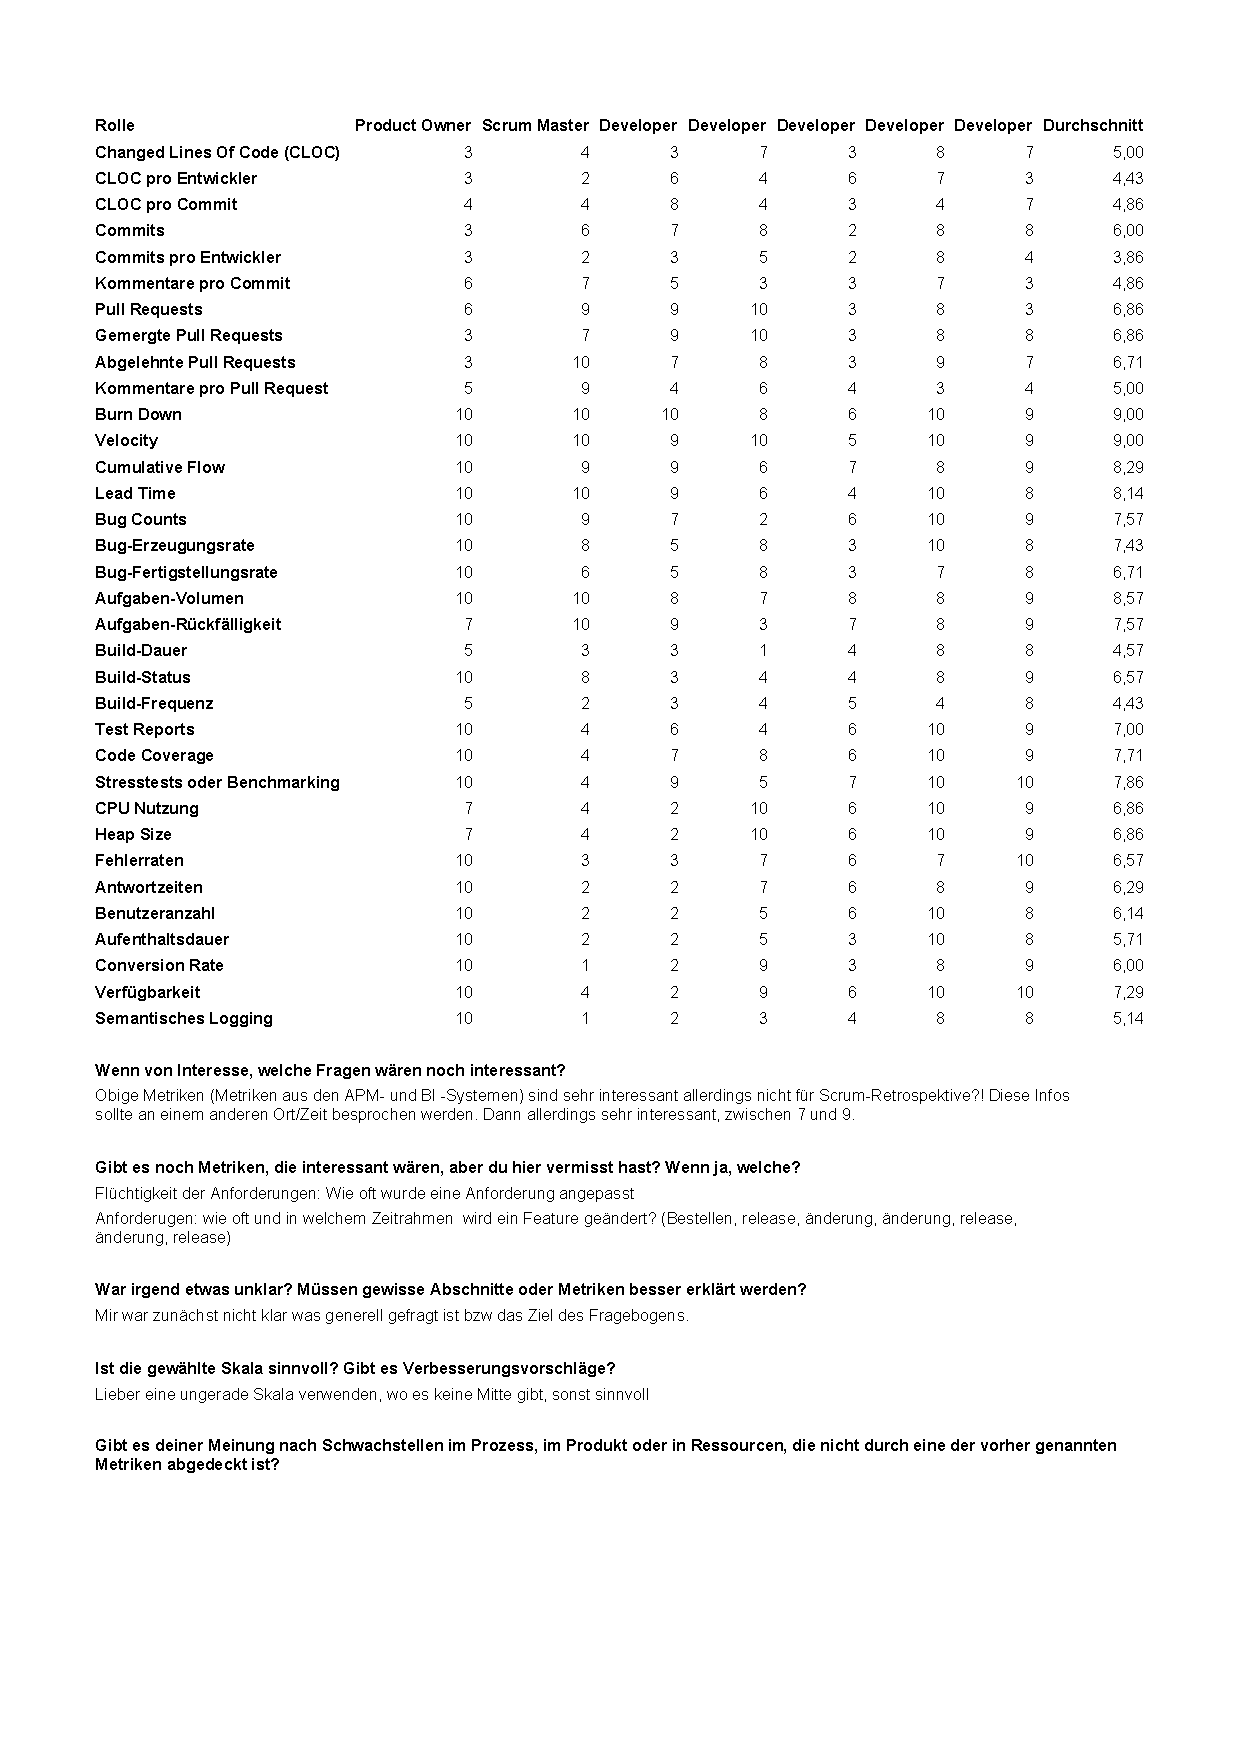
\includepdf[pages=-, scale=0.9, pagecommand={\thispagestyle{plain}}]{appendix/fragebogen-ergebnis.pdf}

\newpage
\section{Transkripte Interviews}\label{appendix:transcript}

Im Folgenden finden sich die Transkripte zu den Interviews, die zu Evaluationszwecken geführt wurden.
Der Interviewer wird mit A und der oder die Interviewte mit B abgekürzt.

\subsection{Product Owner}

A\@: ``Wird das Dashboard von dir genutzt? Wenn ja, wie?'' \\
B\@: ``Bisher primär zur Demonstration, was du in deiner Arbeit gemacht hast. Ich habe es vielen gezeigt, auch darum, um zu zeigen, man kann einfach Daten sammeln und Metriken darstellen. Probleme habe ich teilweise noch mit den Metriken selbst, weil sie nicht alle ausreichend verständlich sind für mich. Uns wären auch noch viele andere eingefallen, beispielsweise zur Darstellung der Testabdeckung der Oberflächentests. Die Herausforderung für die Zukunft wird sein, sinnvolle Metriken finden zu können. Es muss klarer sein, was das Ziel der Metriken ist. Große Probleme hatte ich mit der Acceptance Criteria Volatility. Ich war aufgrund der Zahl irritiert, da ich Prozent gewohnt bin. Diese Metrik muss auch dahingehend verändert werden, dass die Veränderungen erst ab dem Status Prepared gezählt werden, denn davor ist es noch Aufarbeitung der Aufgabe, da kann sich noch viel ändern. Mir war ebenfalls nicht klar, was ist gut, was ist schlecht. Sehr nützlich wäre aus meiner Sicht auch noch eine textuelle Beschreibung der Ziele, die mit den Metriken verfolgt werden. Damit auch in der Retrospektive klar ist, was ist gut gelaufen und was nicht und auch Empfehlungen gegeben werden, wie ein Ziel verbessert werden kann. Ein Beispiel wären die Atlassian Playbooks~\footcite{atlassian_playbook}, die spielerisch versuchen, Probleme im Prozess zu beseitigen.'' \\
A\@: ``Rückblickend gesehen, wurden die richtigen Metriken ermittelt und auf dem Dashboard visualisiert?'' \\
B\@: ``Schwierig zu sagen, für mich ist primär die Acceptance Criteria Volatility interessant, da sie eine Aussage über meine Arbeit trifft. Ein Vorschlag wäre noch, aufzuteilen, für wen welche Metriken interessant sein könnten. Die Einteilung könnte noch etwas klarer sein. Interessant wäre jetzt auch eine Kombination der Metriken, zum Beispiel die Bug Rate kombiniert mit den Releasezyklen. Ich lasse mich überraschen, was der Scrum Master für Ideen hat, weil es grundsätzlich seine Herausforderung sein wird.''

\subsection{Scrum Master}

A\@: ``Ich sehe, du hast schon etwas vorbereitet, du kannst gerne anfangen.'' \\
B\@: ``Ein paar Dinge, die mir aufgefallen sind: Im Dashboard wäre es sehr nützlich, den Zeitraum auf `ab dem letzten Sprint' setzen zu können, das muss jetzt immer manuell als absolutes Datum gesetzt werden. Sinnvoll wäre auch noch, wenn die Generierung der Daten vor Mitternacht passiert, damit sie den Zeitstempel des richtigen Tages haben. Interessant sind auch die Tage, an denen der alte Sprint geschlossen und der neue gestartet wird. Wie es sich dann damit verhaltet. Weiters ist mir noch aufgefallen, dass die Visualisierung bei den Labels nicht sinnvoll ist für unser Team, eine solche Wortwolke ist eher nützlich für das Management, für uns wäre eine Verteilung interessanter, um zu sehen, wie sie sich entwickeln. Bei der Lead Time ist mir aufgefallen, dass ich im Vergleich zum \ac{PTS} noch zu wenig Detailinformationen habe. Für mich sehr nützlich ist die Velocity über die Sprints, weil man sieht, ob sich die geschätzten und erledigten Punkte über eine längeren Zeitraum angleichen. Im \ac{PTS} finden sich noch weitere Metriken, die interessant sein könnten. In Zukunft werden wir auch mit Versionen arbeiten, diese könnten ebenfalls interessant sein im Dashboard, beispielsweise, wie lange wurde an einer Version gearbeitet oder wie viele Entwickler waren beteiligt.'' \\
A\@: ``Wird das Dashboard von dir genutzt? Wenn ja, wie?'' \\
B\@: ``Ich öffne es regelmäßig, für mich sind die Long Term Metrics interessanter, dort betrachte ich meist die letzten 30 Tage, um zu sehen, wie entwickelt sich das Team über die letzten zwei Sprints. Vor allem die Velocity ist hier interessant, eine Trendlinie wäre hier super, um noch besser zu sehen, wie sich die Kennzahlen entwickeln.'' \\
A\@: ``Ist das Dashboard übersichtlich und klar eingeteilt?'' \\
B\@: ``Die Einteilung in Short Term und Long Term Metrics macht auf jeden Fall Sinn, die Anordnung ist für mich okay, mit den Coverage Daten kann ich jetzt weniger anfangen, mit dem Cumulative Flow schon mehr. Wobei wir diesen jeden Tag auf unserem physischen Scrumboard sehen. Kombiniert mit anderen Metriken würde das dann mehr Sinn machen, beispielsweise mit der Bug Rate. Burndown Chart macht in dieser Form auch wenig Sinn, das haben wir im \ac{PTS}, aber auch das macht in Kombination mit anderen Metriken Sinn. Issue Labels könnten als Liniendiagramm dargestellt und in die Long Term Metrics übernommen werden, um Trends erkennbar zu machen. Diese lässt sich dann auch einfacher mit anderen Metriken kombinieren, um Verbindungen herstellen zu können. Sehr interssant sind auch die Aufgaben, die zusätzlich zum Sprint hinzukommen. Generell kann jetzt begonnen werden, gewisse Metriken zu kombinieren, um noch bessere Einsichten in den Prozess zu bekommen.'' \\
A\@: ``Rückblickend gesehen, wurden die richtigen Metriken ermittelt und auf dem Dashboard visualisiert?'' \\
B\@: ``Ja die Metriken sind recht gut gewählt. Je mehr wir sammeln und anzeigen können, desto besser. Aber auch je mehr wir kombinieren können, desto besser.'' \\
A\@: ``Welche Metriken auf dem Dashboard sind besonders nützlich oder werden oft genutzt?'' \\
B\@: ``Für mich sind die Trends in den Long Term Metrics interessanter. Gut wären auch noch detailliertere Ansichten, beispielsweise, wenn ich einen Punkt in einem Diagramm anklicke, dass ich sofort sehe, welche Daten dort dahinter liegen. Derzeit muss ich das dann über das \ac{PTS} ermitteln.'' \\
A\@: ``Ist bereits eine Qualitätsverbesserung im Prozess oder in einem Produkt spürbar? Oder sogar nachweisbar?'' \\
B\@: ``Noch nicht, wir haben es verwendet und alle einmal hinein gesehen, aber momentan ist es noch so, dass wir Daten sammeln, weil mit den zwei oder drei Sprints noch keine klare Aussage getroffen werden kann. Außerdem sind unsere Sprints noch sehr unterschiedlich, wie du sehen kannst.''

\subsection{Entwicklerin}

A\@: ``Wird das Dashboard von dir genutzt? Wenn ja, wann und wie nutzt du das Dashboard?'' \\
B\@: ``Aktuell nutze ich das Dashboard nicht sehr oft, aber wenn ich es nutze, finde ich es sehr hilfreich, dass ich gleich die Code Coverage sehe, so erspare ich mit den Blick ins SonarQube. Auch sehr interessant für mich sind die Anzahl Bugs und zusätzlich aufnehmen könnte man noch die Vulnerabilities aus SonarQube, um den aktuellen Status der Software besser erkennen zu können.'' \\
A\@: ``Ist das Dashboard übersichtlich und klar eingeteilt?'' \\
B\@: ``Aktuell ist die Einteilung für mich klar, ich persönlich würde noch den Cumulative Flow weiter nach unten schieben, da für mich vor allem die Short Term Metrics interessant sind.'' \\
A\@: ``Rückblickend gesehen, wurden die richtigen Metriken ermittelt und auf dem Dashboard visualisiert?'' \\
B\@: ``Ja, in Zukunft kann es noch weiter ausgebaut werden, auch, dass alle Produkte noch detiallierter dargestellt werden.'' \\
A\@: ``Werden Long Term Metrics auch von dir genutzt?'' \\
B\@: ``Interessant finde ich die Velocity, um erkennen zu können, was wir uns vorgenommen haben und was wir wirklich abschließen konnten. Auch die Acceptance Criteria Volatility finde ich sehr interessant, vor allem um den Prozess noch weiter zu verbessern. Hier sind auch die Histogramme hilfreich, um die Verteilung besser erkennen zu können. Für manche war diese Kennzahl verwirrend, da nicht klar war, ob es Prozent sind. Eine bessere Beschreibung wäre hier sinnvoll. Generell werden die Long Term Metrics eher bei den Retrospektiven genutzt.'' \\
A\@: ``Ist bereits eine Qualitätsverbesserung im Prozess oder in einem Produkt spürbar? Oder sogar nachweisbar?'' \\
B\@: ``Mir persönlich ist aufgefallen, dass wir durch den Bug Count frühzeitig gewarnt werden und auch gleich reagieren können.'' \\
A\@: ``Gibt es aus deiner Sicht Verbesserungspotential? Wo liegen aus deiner Sicht die Schwächen dieser Lösung?'' \\
B\@: ``Was mir noch nicht ganz klar ist, bei der Coverage, auf welchen Branch sich das bezieht.'' \\
A\@: ``Die SonarQube Komponente kann bei der Erstellung des Diagramms angegeben werden, in diesem Fall der Master Branch.'' \\
A\@: ``Rückblickend gesehen, wurden die richtigen Metriken ermittelt und auf dem Dashboard visualisiert?'' \\
B\@: ``Ich finde die Short Term Metrics sehr gut gewählt, wie schon gesagt, vermisse ich hier noch die Vulnerabilities aus SonarQube, zumindest für die wichtigsten Komponenten.''


\chapter*{Eidesstattliche Erklärung}
\addcontentsline{toc}{chapter}{Eidesstattliche Erklärung}
Ich erkläre hiermit an Eides statt, dass ich die vorliegende Masterarbeit selbstständig und ohne Benutzung anderer als der angegebenen Hilfsmittel angefertigt habe. Die aus fremden Quellen direkt oder indirekt übernommenen Stellen sind als solche kenntlich gemacht. Die Arbeit wurde bisher weder in gleicher noch in ähnlicher Form einer anderen Prüfungsbehörde vorgelegt und auch noch nicht veröffentlicht.

\vspace{3cm}
\noindent
Dornbirn, am [Tag. Monat Jahr anführen]\hfill [Vor- und Nachname Verfasser/in]


\end{document}
